%!LW recipe=latexmk-xelatex
\documentclass[compress]{beamer}

\usetheme[block=fill]{metropolis}

\usepackage{graphicx} % Allows including images
\usepackage{amsmath,amsfonts,amsthm,amssymb}
\usepackage{color}
\usepackage{xcolor,cancel}
\usepackage[shortlabels]{enumitem}
\setitemize{label=\usebeamerfont*{itemize item}%
	\usebeamercolor[fg]{itemize item}
	\usebeamertemplate{itemize item}}
\definecolor{mDarkBrown}{HTML}{604c38}
\definecolor{mDarkTeal}{HTML}{23373b}
\definecolor{mLightBrown}{HTML}{EB811B}
\definecolor{mMediumBrown}{HTML}{C87A2F}
\definecolor{mygreen}{HTML}{98C2B9}
\definecolor{myyellow}{HTML}{DFD79C}
\definecolor{myblue}{HTML}{8CA7CC}
\definecolor{kern}{HTML}{8CC2B7}


\usepackage{float}
\usepackage{framed}
\usepackage{epsfig}
\usepackage{graphicx}
\usepackage{subcaption}
\usepackage{ulem}
\usepackage{hhline}
\usepackage{multirow}
\usepackage{comment}   
\usepackage{bbm}
\usepackage{tikz}   
\def\Put(#1,#2)#3{\leavevmode\makebox(0,0){\put(#1,#2){#3}}}
\newcommand*\mystrut[1]{\vrule width0pt height0pt depth#1\relax}
\newcommand{\eqdef}{\mathbin{\stackrel{\rm def}{=}}}


\newcommand{\bs}[1]{\boldsymbol{#1}}
\newcommand{\bv}[1]{\mathbf{#1}}
\newcommand{\R}{\mathbb{R}}
\newcommand{\E}{\mathbb{E}}

\DeclareMathOperator*{\argmin}{arg\,min}
\DeclareMathOperator*{\argmax}{arg\,max}
\DeclareMathOperator{\nnz}{nnz}
\DeclareMathOperator{\Var}{Var}
\DeclareMathOperator{\diag}{diag}
\DeclareMathOperator{\sinc}{sinc}
\DeclareMathOperator{\sign}{sign}
\DeclareMathOperator{\dist}{dist}
\DeclareMathOperator{\mv}{mv}
\DeclareMathOperator{\sgn}{sgn}
\DeclareMathOperator{\step}{step}
\DeclareMathOperator{\gap}{gap}
\DeclareMathOperator{\poly}{poly}
\DeclareMathOperator{\tr}{tr}
\DeclareMathOperator{\orth}{orth}
\newcommand{\norm}[1]{\|#1\|}
\captionsetup[subfigure]{labelformat=empty}
\captionsetup[figure]{labelformat=empty}
\DeclareMathOperator*{\lmin}{\lambda_{min}}
\DeclareMathOperator*{\lmax}{\lambda_{max}}

\newcommand{\specialcell}[2][c]{%
  \begin{tabular}[#1]{@{}c@{}}#2\end{tabular}}
\newcommand{\specialcellleft}[2][c]{%
\begin{tabular}[#1]{@{}l@{}}#2\end{tabular}
}

\newtheorem{claim}[theorem]{Claim}

\usepackage{tabstackengine}
\stackMath


%----------------------------------------------------------------------------------------
%	TITLE PAGE
%----------------------------------------------------------------------------------------

\title{CS-GY 6763: Lecture 6 \\ Gradient Descent and Projected Gradient Descent}
\author{NYU Tandon School of Engineering, Prof. Christopher Musco}
\date{}

\begin{document}

\begin{frame}
	\titlepage 
\end{frame}

\metroset{titleformat=smallcaps}

\begin{frame}
	\frametitle{administrative}
	\begin{itemize}
		\item Homework 2 due next Tuesday evening. 
		\item First reading group meeting, \textbf{Monday 3-4pm}. Meet on 11th floor of 370 Jay St. Thank you \textbf{Roman and Marc} for volunteering to present! Please review their chosen paper before the meeting.
		\item Midterm \textbf{next Friday}. 1 hour test, followed by break, then lecture by our TA Feyza on \emph{fine-grained complexity}. I will post midterm review document and practice questions. 
		\begin{itemize}
			\item Nothing from today will be covered on the midterm. 
		\end{itemize}
	\end{itemize}
\end{frame}

\begin{frame}[standout]
	\begin{center}
		finish up lsh + near neighbor search
	\end{center}
\end{frame}

\begin{frame}
	\frametitle{locality sensitive hash functions}
	Let $h: \R^d \rightarrow \{1, \ldots, m\}$ be a random hash function. 
	
	We call $h$ \emph{locality sensitive} for similarity function $s(\bv{q},\bv{y})$ if $\Pr\left[h(\bv{q}) == h(\bv{y})\right]$ is:
	\begin{itemize}
		\item Higher when $\bv{q}$ and $\bv{y}$ are more similar, i.e. $s(\bv{q},\bv{y})$ is higher.
		\item Lower when $\bv{q}$ and $\bv{y}$ are more dissimilar, i.e. $s(\bv{q},\bv{y})$ is lower. 
	\end{itemize}
\begin{center}
	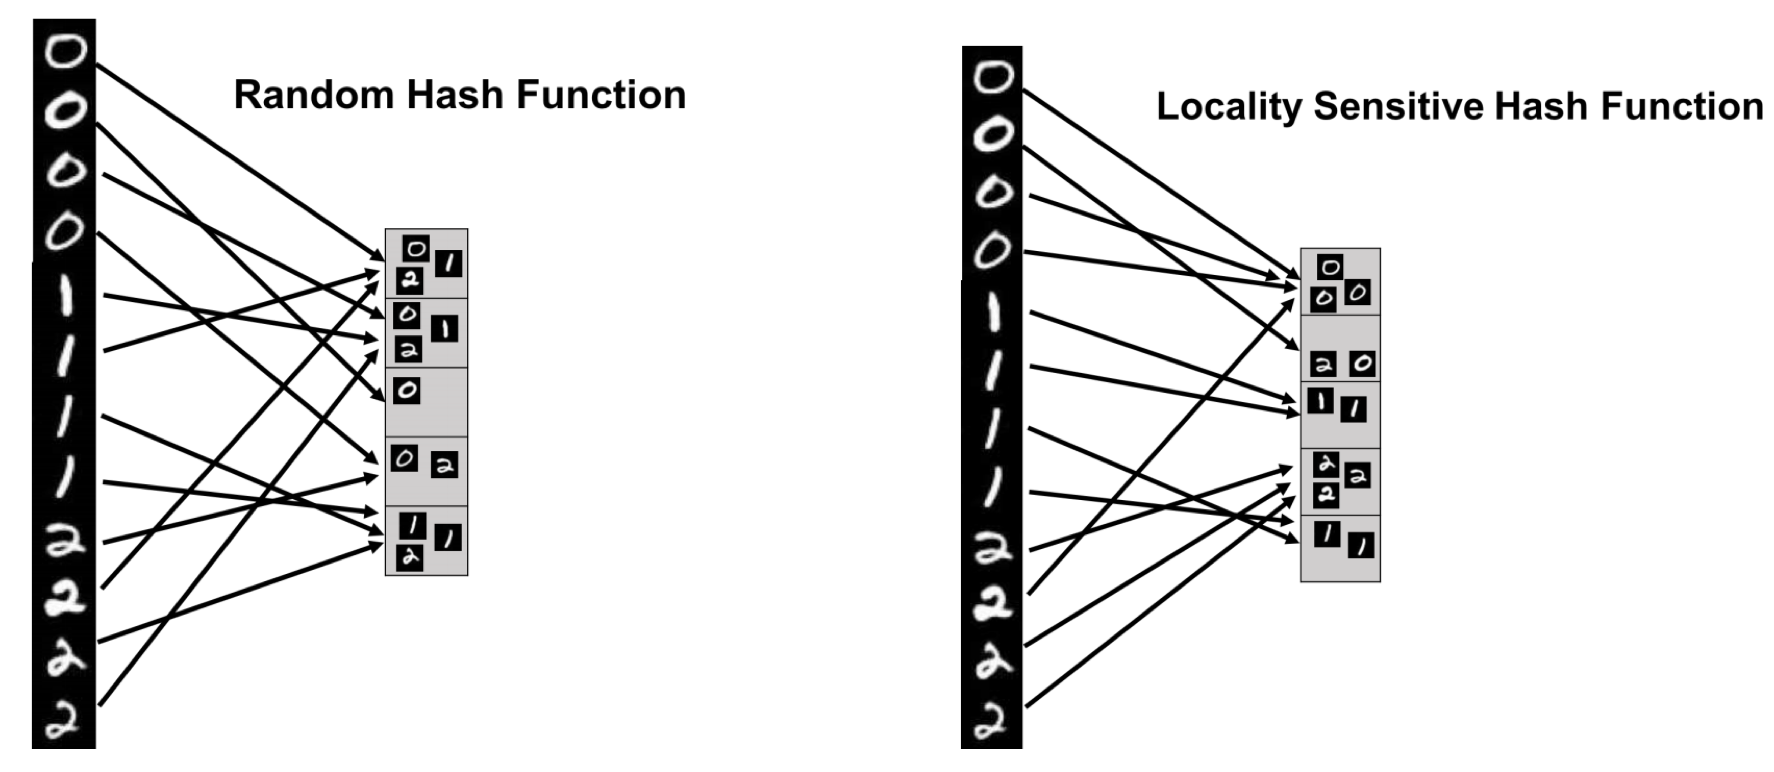
\includegraphics[width=.9\textwidth]{cam_lsh.png}
\end{center}
\end{frame}

\begin{frame}
	\frametitle{other lsh functions}
	\begin{center}
		We saw how MinHash gives an LSH function for Jaccard similarity. Good locality sensitive hash functions exists for other similarity measures.
	\end{center}
	\textbf{Cosine similarity $\cos\left(\theta(\bv{x},\bv{y})\right) = \frac{\langle \bv{x},\bv{y}\rangle}{\|\bv{x}\|_2\|\bv{y}\|_2}$:}
	\begin{center}
		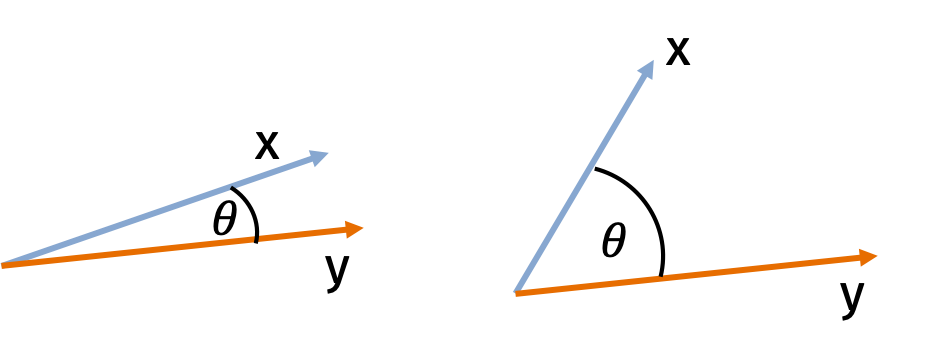
\includegraphics[width=.7\textwidth]{cos_sim.png}
		
		$-1 \leq \cos\left(\theta(\bv{x},\bv{y})\right) \leq 1$.
	\end{center}
\end{frame}

\begin{frame}
	\frametitle{cosine similarity}
	\begin{center}
		Cosine similarity is natural ``inverse" for Euclidean distance.
	\end{center}
		\textbf{Euclidean distance $\|\bv{x} - \bv{y}\|_2^2$:}
		\begin{itemize}
			\item Suppose for simplicity that $\|\bv{x}\|_2^2 = \|\bv{y}\|_2^2 = 1$.
		\end{itemize}
\end{frame}

\begin{frame}
	\frametitle{simhash}
	Locality sensitive hash for \textbf{cosine similarity}:
	\begin{itemize}
		\item Let $\bv{g} \in \R^d$ be randomly chosen with each entry $\mathcal{N}(0,1)$. 
		\item Let $f: \{-1,1\} \rightarrow \{1,\ldots, m\}$ be a uniformly random hash function. 
		\item $h: \R^d \rightarrow \{1,\ldots, m\}$ is definied $h(\bv{x}) = f\left(\sign(\langle \bv{g}, \bv{x} \rangle)\right)$.
	\end{itemize}
	\begin{center}
		\alert{\textbf{
				\large
				Claim: If $\cos(\theta(\bv{x},\bv{y})) = v$, then $$\Pr[h(\bv{x}) == h(\bv{y})] = 1 - \frac{\theta}{\pi}  + \frac{1-v}{m}$$.
		}}
	\end{center}
\end{frame}


%\begin{frame}
%	\frametitle{simhash}
%	\begin{center}
%		\textbf{Inspired by Johnson-Lindenstrauss sketching}
%		
%		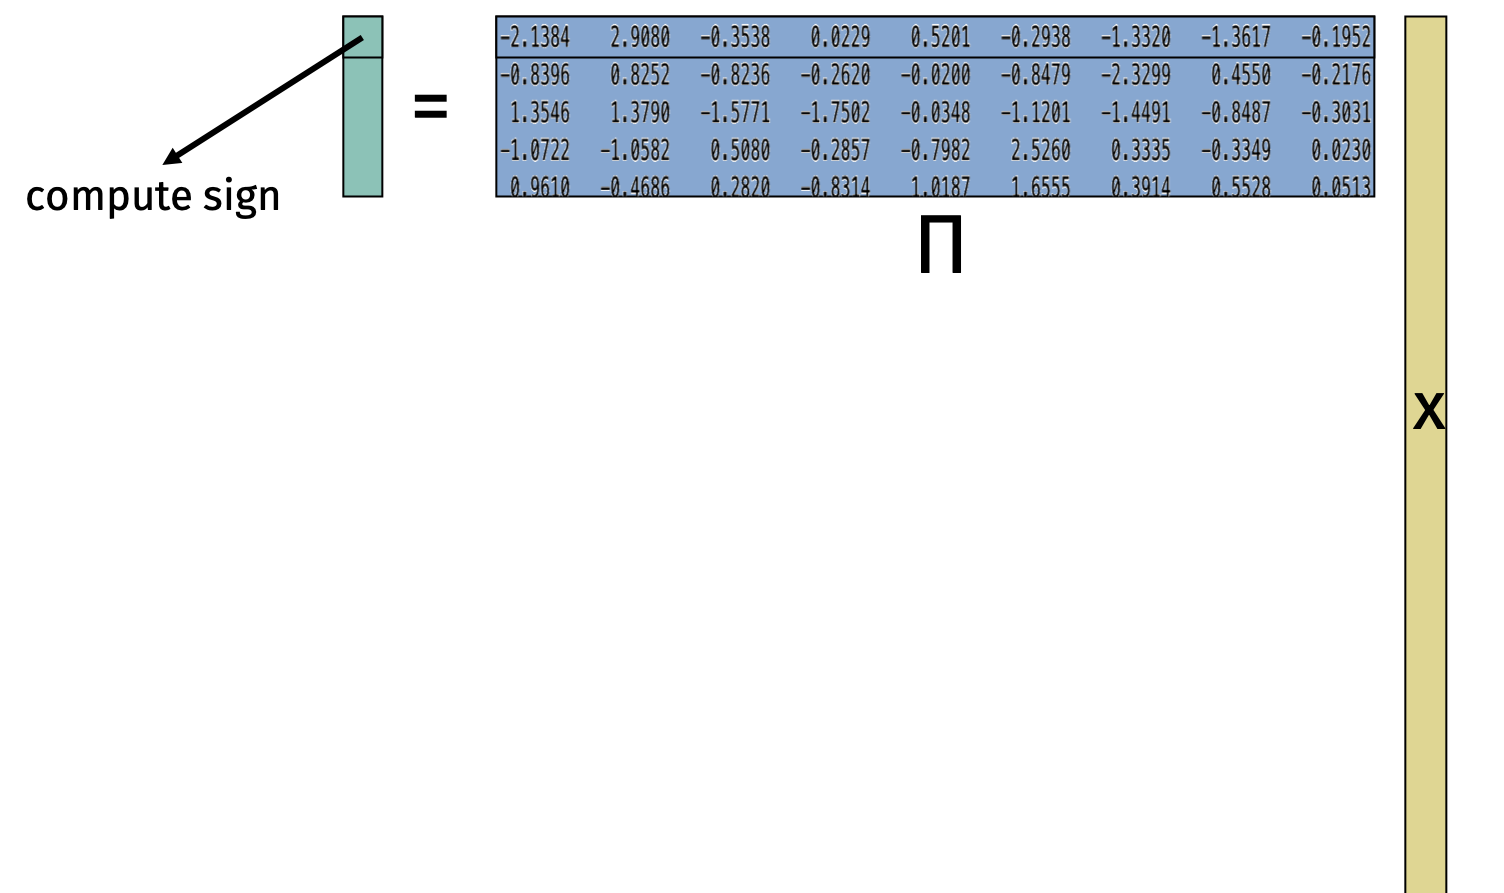
\includegraphics[width=\textwidth]{simhash_jl.png}
%	\end{center}
%\end{frame}



\begin{frame}[t]
	\frametitle{simhash analysis in 2d}
	\textbf{Lemma to prove:} If $\cos(\theta(\bv{x},\bv{y})) = v$, then 
	\begin{align*}
		\Pr[g(\bv{x}) == g(\bv{y})] = 1 - \frac{\theta}{\pi}= 1 - \frac{\cos^{-1}(v)}{\pi}
	\end{align*}
	\begin{center}
		\vspace{-.5em}
		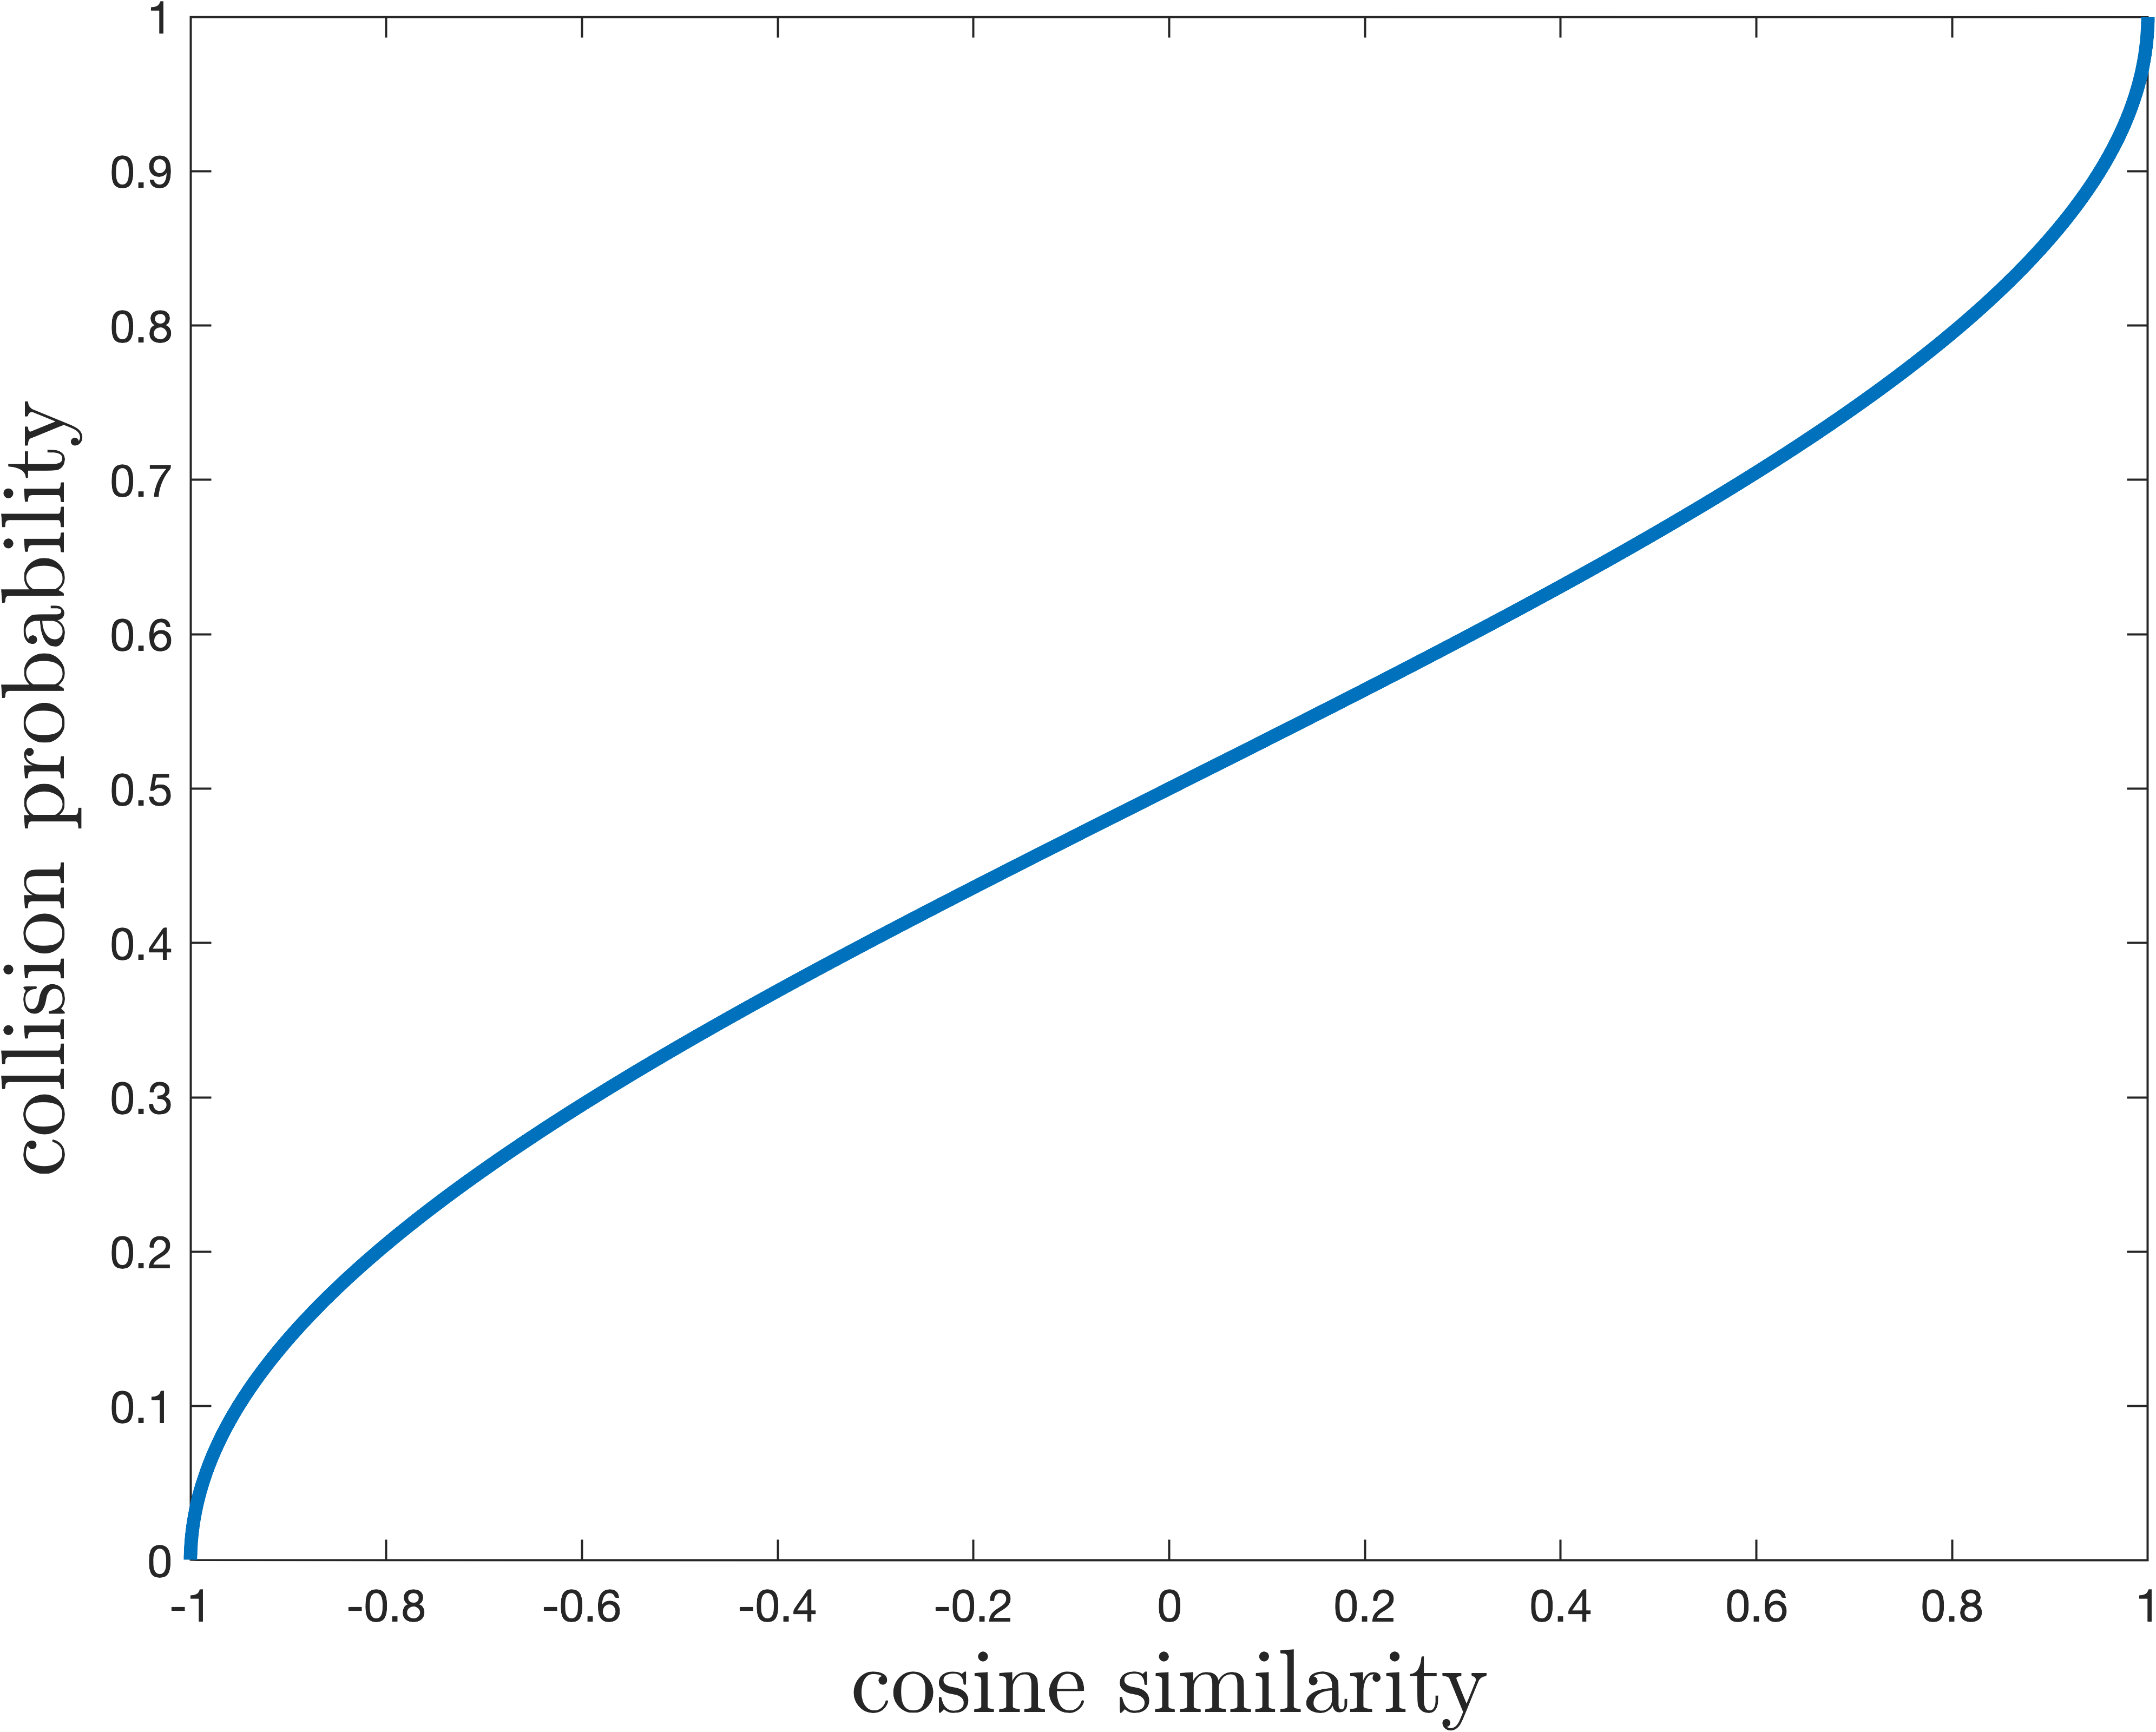
\includegraphics[width=.6\textwidth]{cosine_sim.png}
		$\Pr[h(\bv{x}) == h(\bv{y})] = \Pr[g(\bv{x}) == g(\bv{y})] + \frac{1-v}{m}$.
	\end{center}
\end{frame}

\begin{frame}
	\frametitle{simhash}
	SimHash can be tuned, just like MinHash-based LSH function for Jaccard similarity. Version of hash function with $r$ bands:
	\begin{itemize}
		\item Let $\bv{g}_1,\ldots, \bv{g}_r \in \R^d$ be chosen with each entry $\mathcal{N}(0,1)$. 
		\item Let $f: \{-1,1\}^r \rightarrow \{1,\ldots, m\}$ be a uniformly random hash function. 
		\item $h: \R^d \rightarrow \{1,\ldots, m\}$ is defined $$h(\bv{x}) = f\left([\sign(\langle \bv{g}_1, \bv{x} \rangle),\ldots, \sign(\langle \bv{g}_r, \bv{x} \rangle)]\right)$$.
	\end{itemize}
\begin{align*}
	\Pr[h(\bv{x}) == h(\bv{y})] = \left(1-\frac{\theta}{\Pi}\right)^r
\end{align*}
\end{frame}

\begin{frame}
	\frametitle{simhash analysis 2d}
	\textbf{To prove:}  $\Pr[g(\bv{x}) == g(\bv{y})] = 1 - \frac{\theta}{\pi}$,  where $g(\bv{x}) = \sign(\langle \bv{g}, \bv{x} \rangle)$.
	\vspace{-.5em}
	\begin{center}
		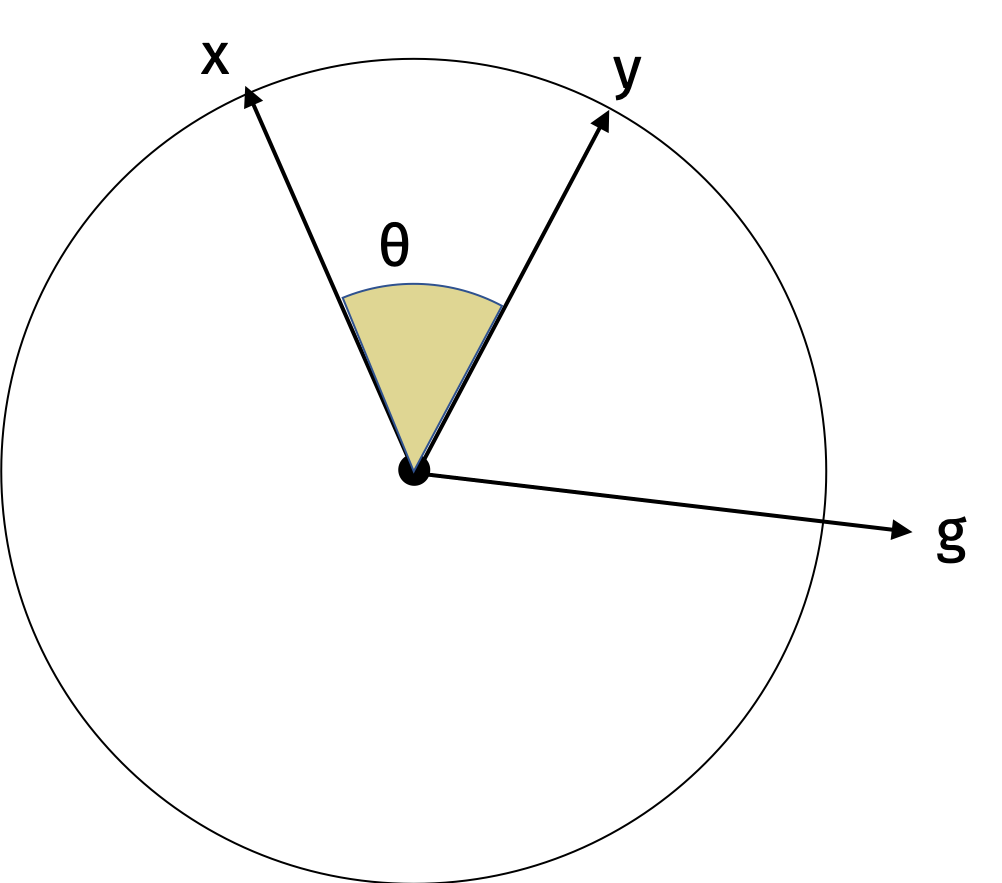
\includegraphics[width=.5\textwidth]{simhash1.png}
	\end{center}
	$\Pr[g(\bv{x}) == g(\bv{y})] = \Pr[\sign(\langle \bv{g}, \bv{x} \rangle) == \sign(\langle \bv{g}, \bv{y} \rangle)] = $ probability  $\bv{x}$ and $\bv{y}$ are on the same side of hyperplane orthogonal to $\bv{g}$.
\end{frame}

\begin{frame}
	\frametitle{simhash analysis higher dimensions}
	\begin{center}
		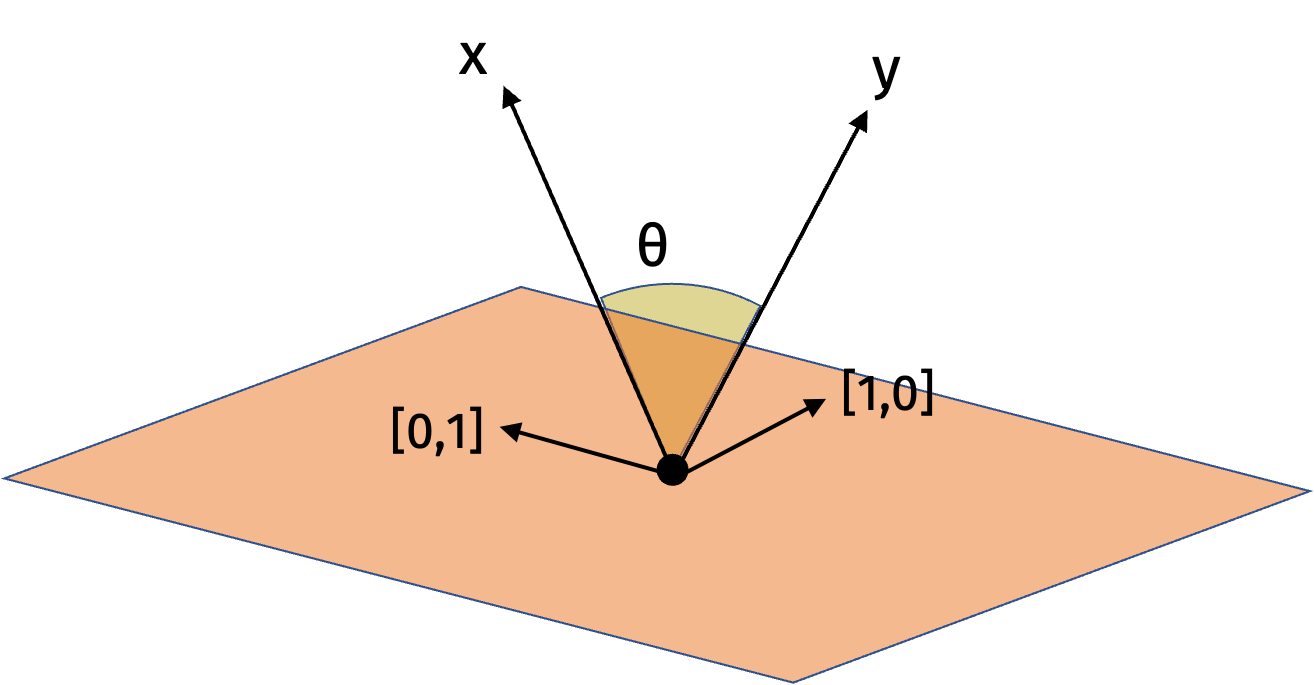
\includegraphics[width=.7\textwidth]{high_dim1.png}
	\end{center}
There is always some \emph{rotation matrix} $\bv{U}$ such that $\bv{U}\bv{x},\bv{U}\bv{y}$ are spanned by the first two-standard basis vectors and have the same cosine similarity as $\bv{x}$ and $\bv{y}$.
\end{frame}

\begin{frame}
	\frametitle{simhash analysis higher dimensions}
	\begin{center}
		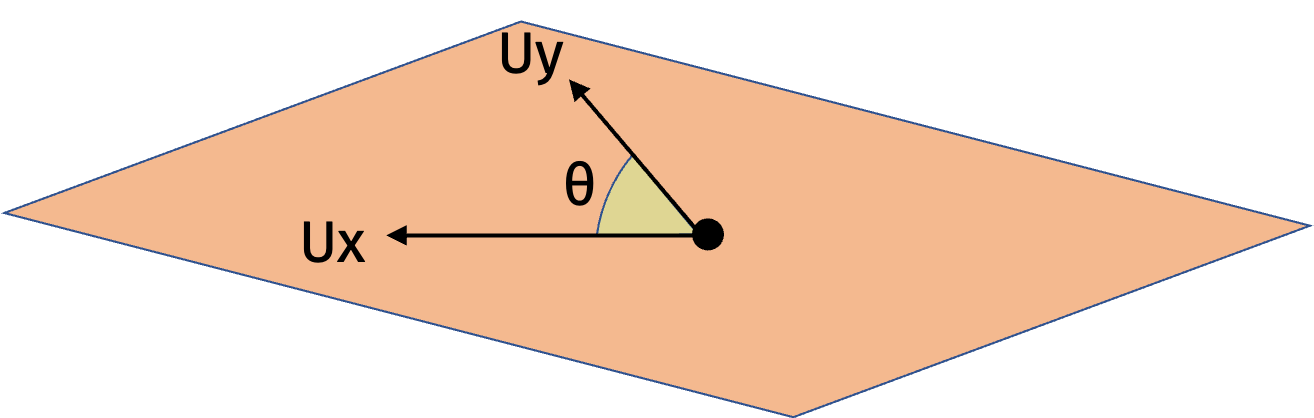
\includegraphics[width=.7\textwidth]{high_dim2.png}
	\end{center}
	There is always some \emph{rotation matrix} $\bv{U}$ such that $\bv{x},\bv{y}$ are spanned by the first two-standard basis vectors. 
	
	
	\textbf{Note:} A rotation matrix $\bv{U}$ has the property that $\bv{U}^T\bv{U} = \bv{I}$. I.e., $\bv{U}^T$ is a rotation matrix itself, which reverses the rotation of $\bv{U}$.
\end{frame}

\begin{frame}[t]
	\frametitle{simhash analysis higher dimensions}
\textbf{Claim:} 
\begin{align*}
	\Pr[\sign(&\langle \bv{g}, \bv{x} \rangle) == \sign(\langle \bv{g}, \bv{y} \rangle)] \\
	&= \Pr[\sign(\langle \bv{g}, \bv{U}\bv{x} \rangle) == \sign(\langle \bv{g}, \bv{U}\bv{y} \rangle)]\\
	&= \Pr[\sign(\langle \bv{g}[1,2], (\bv{U}\bv{x})[1,2] \rangle) == \sign(\langle \bv{g}[1,2], (\bv{U}\bv{y}[1,2] \rangle)] \\
	&= 	1 - \frac{\theta}{\pi}
	\end{align*}
\end{frame}

\begin{frame}
	\frametitle{worst case theoretical result}

	\begin{center}
	Last class and on the homework, we show how to build LSH data structures for specific point sets that achieves $o(n)$ search time by using $\Omega(n)$ space. However, we did't prove any ``worst-case'' theoretical guarantees. 
	\end{center}

	Such guarantees can be proven, and were actually a major driving force in the development of LSH methods.

\end{frame}


\begin{frame}
	\frametitle{worst case theoretical result}
	\begin{center}
	\textbf{\emph{Near Neighbor} Search Problem.}
\end{center}
	\begin{theorem}[Indyk, Motwani, 1998]
		If there exists some $q$ with $\|\bv{q} - \bv{y}\|_0 \leq R$, return a vector $\tilde{\bv{q}}$ with $\|\tilde{\bv{q}} - \bv{y}\|_0 \leq C\cdot R$ in:
		\begin{itemize}
			\item Time: $O\left(n^{1/C}\right)$.
			\item Space: $O\left(n^{1 + 1/C}\right)$. 
		\end{itemize}
	\end{theorem}
	$\|\bv{q} - \bv{y}\|_0 = $ ``hamming distance" = number of elements that differ between $\bv{q}$ and $\bv{y}$. 

	$R$ is a fixed parameter given as part of the input.
\end{frame}

\begin{frame}
	
	\frametitle{approximate nearest neighbor search}
	Exponential search over values of $R$ easily yields:  
		\begin{theorem}[Indyk, Motwani, 1998]
		Let $q$ be the closest database vector to $\bv{y}$. Return a vector $\tilde{\bv{q}}$ with $\|\tilde{\bv{q}} - \bv{y}\|_0 \leq C\cdot \|{\bv{q}} - \bv{y}\|_0$ in:
		\begin{itemize}
			\item Time: $\tilde{O}\left(n^{1/C}\right)$.
			\item Space: $\tilde{O}\left(n^{1 + 1/C}\right)$. 
		\end{itemize}
	\end{theorem}
\end{frame}


\begin{frame}[standout]
	\begin{center}
		optimization
	\end{center}
\end{frame}


\begin{frame}
		\frametitle{continuous optimization}
		Given function $f: \R^d \rightarrow \R$. Find $\hat{\bv{x}}$ such that: 
		\begin{align*}
			f(\hat{\bv{x}}) \leq \min_{\bv{x}}f(\bv{x}) + \epsilon.
		\end{align*}
\end{frame}

\begin{frame}
	\frametitle{next unit: continuous optimization}
	Have some function $f : \R^d \rightarrow \R$. Want to find ${\bv{x}}^*$ such that:
	\begin{align*}
		f({\bv{x}}^*) = \min_{\bv{x}} f(\bv{x}).
	\end{align*}
	Or at least $\hat{\bv{x}}$ which is close to a minimum. E.g. $f(\hat{\bv{x}}) \leq \min_{\bv{x}} f(\bv{x}) + \epsilon$
	
	Often we have some additional constraints:
	\begin{itemize}
		\item $\bv{x} > 0$.
		\item $\|\bv{x}\|_2 \leq R$, $\|\bv{x}\|_1 \leq R$.
		\item $\bv{a}^T\bv{x} > c$.
	\end{itemize}
\end{frame}

\begin{frame}
	\frametitle{continuous optimization}
	\textbf{Dimension $d = 1$:}
	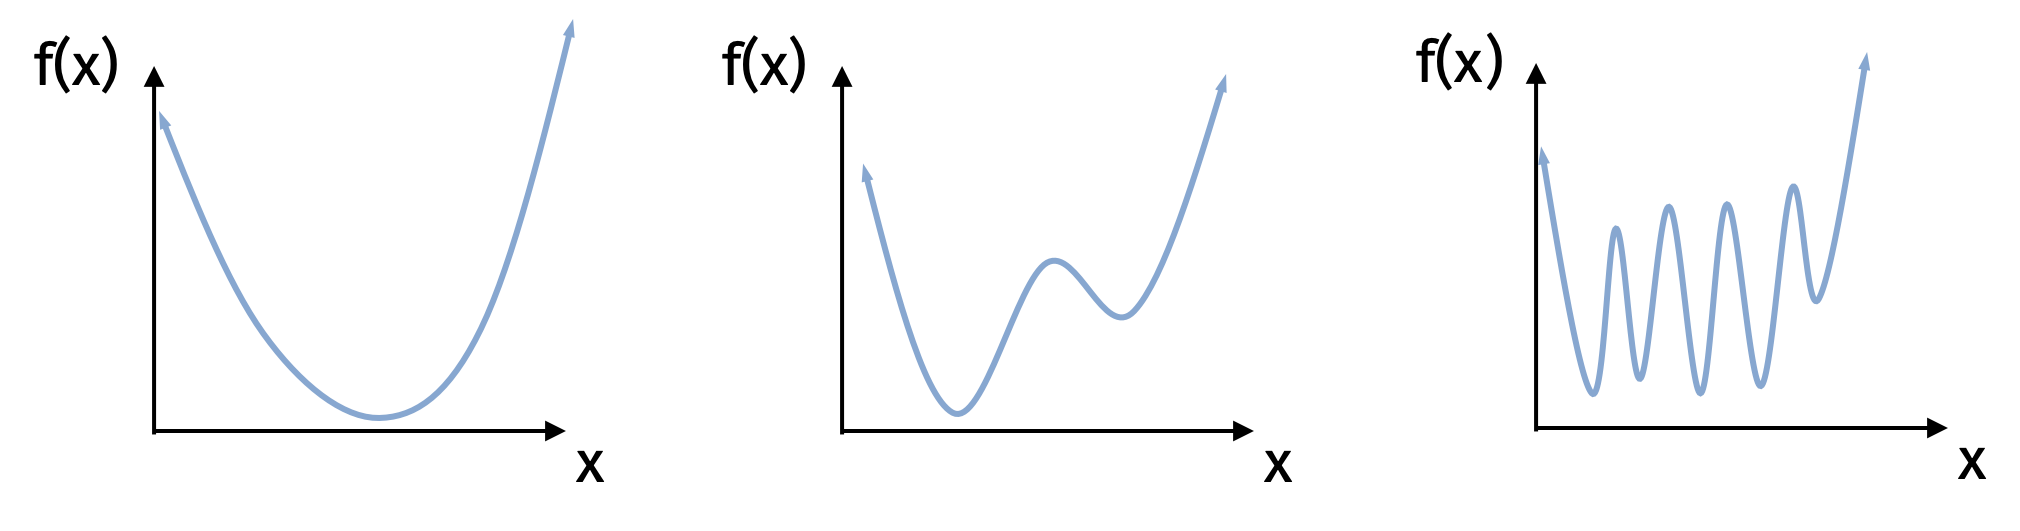
\includegraphics[width=\textwidth]{1d_functions.png}
	
	\textbf{Dimension $d = 2$:}
	
	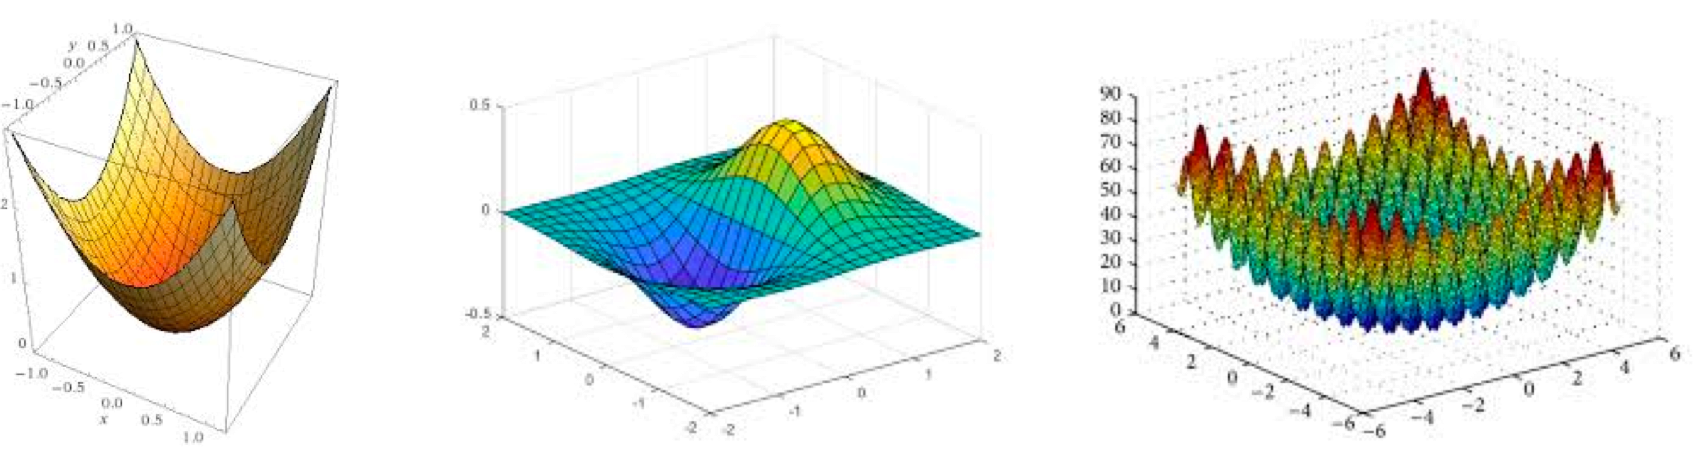
\includegraphics[width=\textwidth]{2dfunctions.png}
\end{frame}

\begin{frame}
	\frametitle{optimization in machine learning}
	\begin{center}
		\alert{\textbf{Continuouos optimization is the foundation of modern machine learning.}}
	\end{center}
	\textbf{Supervised learning:} Want to learn a model that maps \emph{inputs}
	\begin{itemize}
		\item numerical data vectors
		\item images, video
		\item text documents
	\end{itemize} 
	
	to \emph{predictions}
	\begin{itemize}
		\item numerical value (probability stock price increases)
		\item label (is the image a cat? does the image contain a car?)
		\item decision (turn car left, rotate robotic arm)
	\end{itemize} 
\end{frame}

\begin{frame}
	\frametitle{machine learning model}
	\begin{center}
		Let $M_{\bv{x}}$ be a model with parameters $\bv{x} = \{x_1, \ldots, x_k\}$, which takes as input a data vector $\bv{a}$ and outputs a prediction.
	\end{center}
	
	\textbf{Example:}
	\begin{align*}
		M_{\bv{x}}(\bv{a}) = \sign(\bv{a}^T\bv{x})
	\end{align*}		
\end{frame}

\begin{frame}[t]
	\frametitle{machine learning model}
	\textbf{Example:}
	\begin{center}
		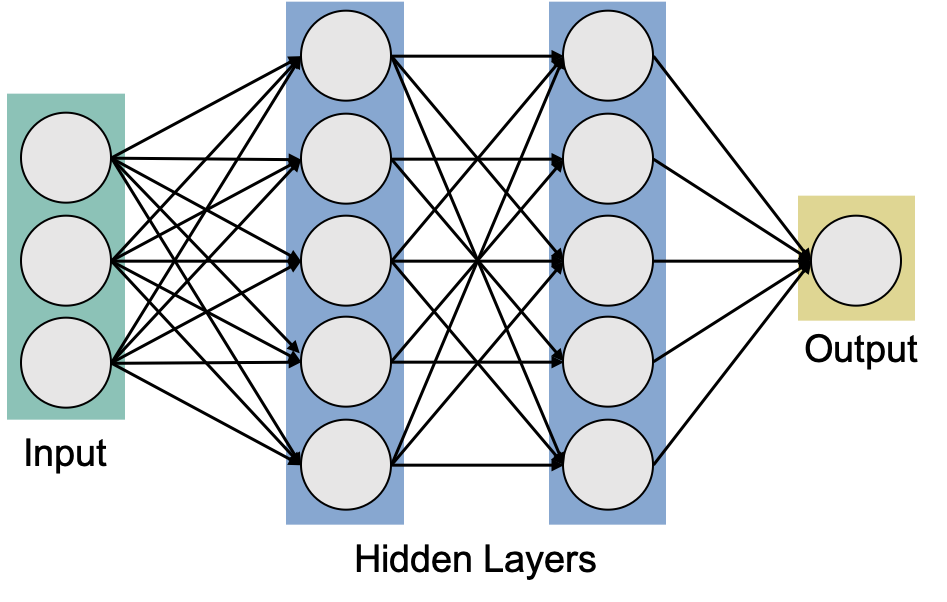
\includegraphics[width=.7\textwidth]{neuralNetwork.png}
	\end{center}	
	$\bv{x}\in \R^{\text{(\# of connections)}}$ is the parameter vector containing all the network weights. 	
\end{frame}

\begin{frame}
	\frametitle{supervised learning}
	Classic approach in \emph{supervised learning}: Find a model that works well on data that you already have the answer for (labels, values, classes, etc.).
	\begin{itemize}
		\item Model $M_{\bv{x}}$ parameterized by a vector of numbers $\bv{x}$.
		\item Dataset $\bv{a}^{(1)}, \ldots,  \bv{a}^{(n)}$ with outputs $y^{(1)}, \ldots, y^{(n)}$.
	\end{itemize}
	\begin{center}
		Want to find $\hat{\bv{x}}$ so that $M_{\hat{\bv{x}}}(\bv{a}^{(i)}) \approx y^{(i)}$ for $i \in 1,\ldots, n$.
		
		\alert{\textbf{How do we turn this into a function minimization problem?}}
	\end{center}
\end{frame}

\begin{frame}
	\frametitle{loss function}
	\textbf{Loss function $L\left(M_{\bv{x}}(\bv{a}), y\right)$:} Some measure of distance between prediction $M_{\bv{x}}(\bv{a})$ and target output $y$. Increases if they are further apart.
	\begin{itemize}
		\item Squared ($\ell_2$) loss: $|M_{{\bv{x}}}(\bv{a}) - y|^2$
		\item Absolute deviation ($\ell_1$) loss: $|M_{{\bv{x}}}(\bv{a}) - y|$
		\item Hinge loss: 1 - $y \cdot M_{{\bv{x}}}(\bv{a})$ 
		\item Cross-entropy loss (log loss). 
		%		$−o  \log(M_{{\bv{x}}}(\bv{y})+(1 - o)\log(1 - M_{{\bv{x}}}(\bv{y}))$
		\item Etc.
	\end{itemize}
\end{frame}

\begin{frame}
	\frametitle{empirical risk minimization}
	\textbf{Empirical risk minimization}:
	\begin{align*}
		f(\bv{x}) = \sum_{i=1}^n L\left(M_{\bv{x}}(\bv{a}^{(i)}), y^{(i)}\right)
	\end{align*}
	\begin{center}
		Solve the optimization problem $\min_{\bv{x}} f(\bv{x})$.
	\end{center}
\end{frame}

\begin{frame}
	\frametitle{example: least squares regression}
	\begin{itemize}
		\item $M_{\bv{x}}(\bv{a}) = \bv{x}^T\bv{a}$. $\bv{x}$ contains the regression coefficients. 
		\item $L(z,y) = |z-y|^2$. 
		\item $f(\bv{x}) = \sum_{i=1}^n |\bv{x}^T\bv{a}^{(i)} - y^{(i)}|^2$
	\end{itemize}
	\begin{align*}
		f(\bv{x}) = \|\bv{A}\bv{x} - \bv{y}\|_2^2
	\end{align*}
	where $\bv{A}$ is a matrix with $\bv{a}^{(i)}$ as its $i^\text{th}$ row and $\bv{y}$ is a vector with $y^{(i)}$ as its $i^\text{th}$ entry. 
\end{frame}

\begin{frame}
	\frametitle{algorithms for continuous optimization}
	The choice of algorithm to minimize $f(\bv{x})$ will depend on:
	\begin{itemize}
		\item The form of $f(\bv{x})$ (is it linear, is it quadratic, does it have finite sum structure, etc.)
		\item If there are any additional constraints imposed on $\bv{x}$. E.g. $\|\bv{x}\|_2 \leq c$. 
	\end{itemize}
	\textbf{What are some example algorithms for continuous optimization?}
	
\end{frame}

\begin{frame}
	\frametitle{first topic: gradient descent + variants}
	\textbf{Gradient descent:} A greedy algorithm for minimizing functions of multiple variables that often works amazingly well. 
	\begin{center}
		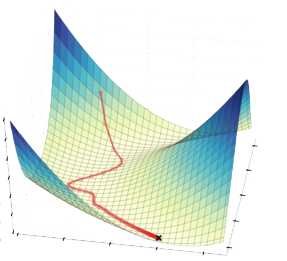
\includegraphics[width=.4\textwidth]{greedy_gradient.png}
		
		Runtime generally scales \emph{linearly} with the dimension of $\bv{x}$ (although this is a bit of an over-simplification).
	\end{center}
\end{frame}

\begin{frame}
	\frametitle{second topic: methods suitable for lower dimension }
	\begin{itemize}
		\item Cutting plane methods (e.g. center-of-gravity, ellipsoid)
		\item Interior point methods
	\end{itemize}
	Fast and more accurate in low-dimensions, slower in very high dimensions. Generally runtime scales \emph{polynomially} with the dimension of $\bv{x}$.
\end{frame}

\begin{frame}
	\frametitle{calculus review}
	For $i = 1, \ldots, d$, let $x_i$ be the $i^\text{th}$ entry of $\bv{x}$. Let $\bv{e}^{(i)}$ be the $i^\text{th}$ \emph{standard basis vector.}
	\vspace{2em}
	
	\textbf{Partial derivative:}
	\begin{align*}
		\frac{\partial f}{\partial x_i}(\bv{x}) = \lim_{t\rightarrow 0} \frac{f(\bv{x} + t\bv{e}^{(i)}) - f(\bv{x})}{t}
	\end{align*}
	\textbf{Directional derivative:}
	\begin{align*}
		D_\bv{v}f(\bv{x}) = \lim_{t\rightarrow 0} \frac{f(\bv{x} + t\bv{v}) - f(\bv{x})}{t}
	\end{align*}
\end{frame}

\begin{frame}
	\frametitle{calculus review}
	\textbf{Gradient}:
	\begin{align*}
		\nabla f(\bv{x}) = 
		\begin{bmatrix}
			\frac{\partial f}{\partial x_1}(\bv{x}) \\ \frac{\partial f}{\partial x_2}(\bv{x}) \\ \vdots \\ \frac{\partial f}{\partial x_d}(\bv{x}) 
		\end{bmatrix}
	\end{align*}
	\textbf{Directional derivative:}
	\begin{align*}
		D_\bv{v}f(\bv{x}) = \lim_{t\rightarrow 0} \frac{f(\bv{x} + t\bv{v}) - f(\bv{x})}{t} = \alert{\nabla f(\bv{x})^T \bv{v}.}
	\end{align*}
\end{frame}


\begin{frame}
	\frametitle{first order optimization}
	Given a function $f$ to minimize, assume we have:
	\begin{itemize}
		\item \textbf{Function oracle}: Evaluate $f(\bv{x})$ for any $\bv{x}$. 
		\item \textbf{Gradient oracle}: Evaluate $\nabla f(\bv{x})$ for any $\bv{x}$.
	\end{itemize}
	We view the implementation of these oracles as black-boxes, but they can often require a fair bit of computation. 
\end{frame}

\begin{frame}[t]
	\frametitle{example gradient evaluation}
	\textbf{Linear least-squares regression}:
	\begin{itemize}
		\item Given $\bv{a}^{(1)}, \ldots \bv{a}^{(n)} \in \R^d$, ${y}^{(1)}, \ldots {y}^{(n)} \in \R$.
		\item Want to minimize:
		\begin{align*}
			f(\bv{x}) = \sum_{i=1}^n \left(\bv{x}^T\bv{a}^{(i)} - {y}^{(i)}\right)^2 = \|\bv{A}\bv{x} - \bv{y}\|_2^2.
		\end{align*} 
	\end{itemize}
	\textbf{What is the time complexity to implement a function oracle for $f(\bv{x})$?}
\end{frame}

\begin{frame}[t]
	\frametitle{example gradient evaluation}
	\textbf{Linear least-squares regression}:
	\begin{itemize}
		\item Want to minimize:
		\begin{align*}
			f(\bv{x}) = \sum_{i=1}^n \left(\bv{x}^T\bv{a}^{(i)} - {y}^{(i)}\right)^2 = \|\bv{A}\bv{x} - \bv{y}\|_2^2.
		\end{align*} 
	\end{itemize}
	
	\begin{align*}
		\frac{\partial f}{\partial x_j} = \sum_{i=1}^n 2\left(\bv{x}^T\bv{a}^{(i)} - {y}^{(i)}\right)\cdot a^{(i)}_j = 2{\bs{\alpha}^{(j)}}^T(\bv{A}\bv{x} -\bv{y})
	\end{align*}
	where $\bs{\alpha}^{(j)}$ is the $j^\text{th}$ \emph{column} of $\bv{A}$. 
\end{frame}

\begin{frame}[t]
	\frametitle{example gradient evaluation}
	\textbf{Linear least-squares regression}:
	\begin{align*}
		\frac{\partial f}{\partial x_j} = \sum_{i=1}^n 2\left(\bv{x}^T\bv{a}^{(i)} - {y}^{(i)}\right)\cdot a^{(i)}_j = 2{\bs{\alpha}^{(j)}}^T(\bv{A}\bv{x} -\bv{y})
	\end{align*}
	where $\bs{\alpha}^{(j)}$ is the $j^\text{th}$ \emph{column} of $\bv{A}$. 
	\begin{align*}
		\nabla f(\bv{x}) = 2\bv{A}^T\left(\bv{A}\bv{x} - \bv{y}\right)
	\end{align*}
	\textbf{What is the time complexity of a gradient oracle for $\nabla f(\bv{x})$?}
\end{frame}

\begin{frame}
	\frametitle{decent methods}
	\textbf{Greedy approach:} Given a starting point $\bv{x}$, make a small adjustment that decreases $f(\bv{x})$. In particular, $\bv{x} \leftarrow \bv{x} + \eta\bv{v}$.
	
	\begin{center}
		\alert{What property do I want in $\bv{v}$?}
	\end{center}
	
	
	\textbf{Leading question:} When $\eta$ is small, what's an approximation for $f(\bv{x} + \eta\bv{v}) - f(\bv{x})$?
	\begin{align*}
		f(\bv{x} + \eta\bv{v}) - f(\bv{x}) \approx \hspace{6em}
	\end{align*}
	
	
\end{frame}

\begin{frame}[t]
	\frametitle{directional derivatives}
	
	\begin{align*}
		D_\bv{v}f(\bv{x}) = \lim_{t\rightarrow 0} \frac{f(\bv{x} + t\bv{v}) - f(\bv{x})}{t} = \nabla f(\bv{x})^T \bv{v}.
	\end{align*}	
	So:
	\begin{align*}
		f(\bv{x} + \eta\bv{v}) - f(\bv{x}) \approx \eta \cdot \nabla f(\bv{x})^T \bv{v}.
	\end{align*}
	
	\textbf{How should we choose $\bv{v}$ so that $f(\bv{x} + \eta\bv{v}) < f(\bv{x})$?} 
	
\end{frame}

\begin{frame}
	\frametitle{gradient descent}
	\textbf{Prototype algorithm:}
	\begin{itemize}
		\item Choose starting point $\bv{x}^{(0)}$.
		\item For $i = 0,\ldots, T$:
		\begin{itemize}
			\item $\bv{x}^{(i+1)} = \bv{x}^{(i)} - \eta \nabla f(\bv{x}^{(i)})$
		\end{itemize}
		\item Return $\bv{x}^{(T)}$.
	\end{itemize}
	
	$\eta$ is a step-size parameter, which is often adapted on the go. For now, assume it is fixed ahead of time.
\end{frame}

\begin{frame}[t]
	\frametitle{gradient descent intuition}
	\textbf{1 dimensional example:}
\end{frame}

\begin{frame}[t]
	\frametitle{gradient descent intuition}
	\textbf{2 dimensional example:}
	\begin{center}
		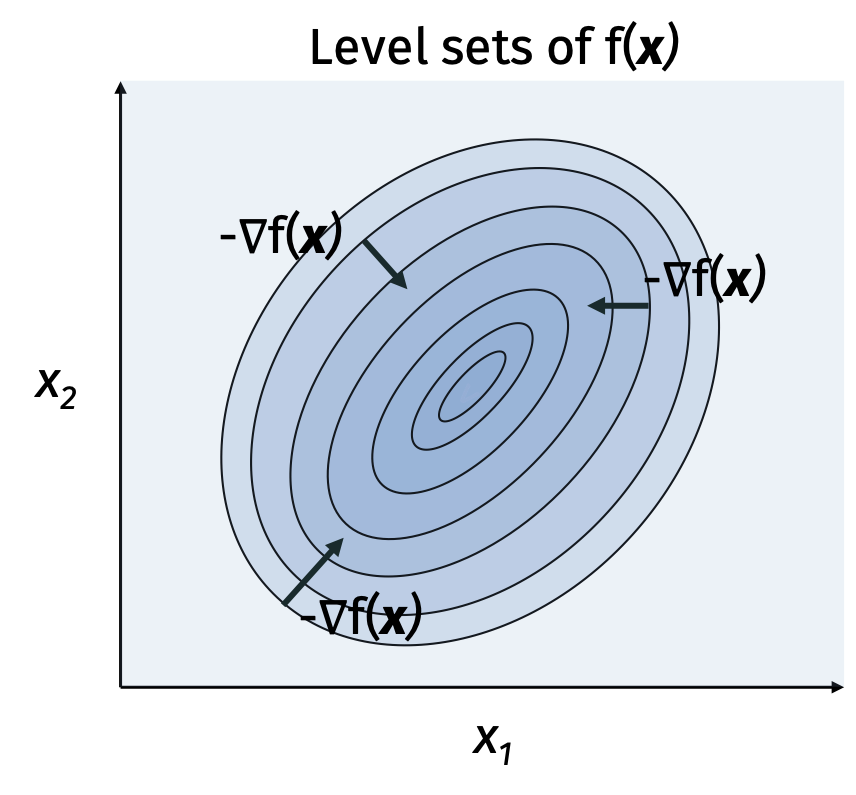
\includegraphics[width=.7\textwidth]{2d_example.png}
	\end{center}
\end{frame}

\begin{frame}[t]
	\frametitle{key results}
	\textbf{For a convex function $f(\bv{x})$:}
	For sufficiently small $\eta$ and a sufficiently large number of iterations $T$, gradient descent will converge to a \alert{\textbf{near global minimum}}:
	\begin{align*}
		f(\bv{x}^{(T)}) \leq  f(\bv{x}^{*}) + \epsilon.  
	\end{align*}
	Examples: least squares regression, logistic regression, kernel regression, SVMs.
	
	\textbf{For a non-convex function $f(\bv{x})$:}
	For sufficiently small $\eta$ and  a sufficiently large number of iterations $T$, gradient descent will converge to a \alert{\textbf{near stationary point}}:
	\begin{align*}
		\|\nabla f(\bv{x}^{(T)})\|_2 \leq  \epsilon.  
	\end{align*}
	Examples: neural networks, matrix completion problems, mixture models. 	
\end{frame}

\begin{frame}[t]
	\frametitle{convex vs. non-convex}
	\begin{center}
		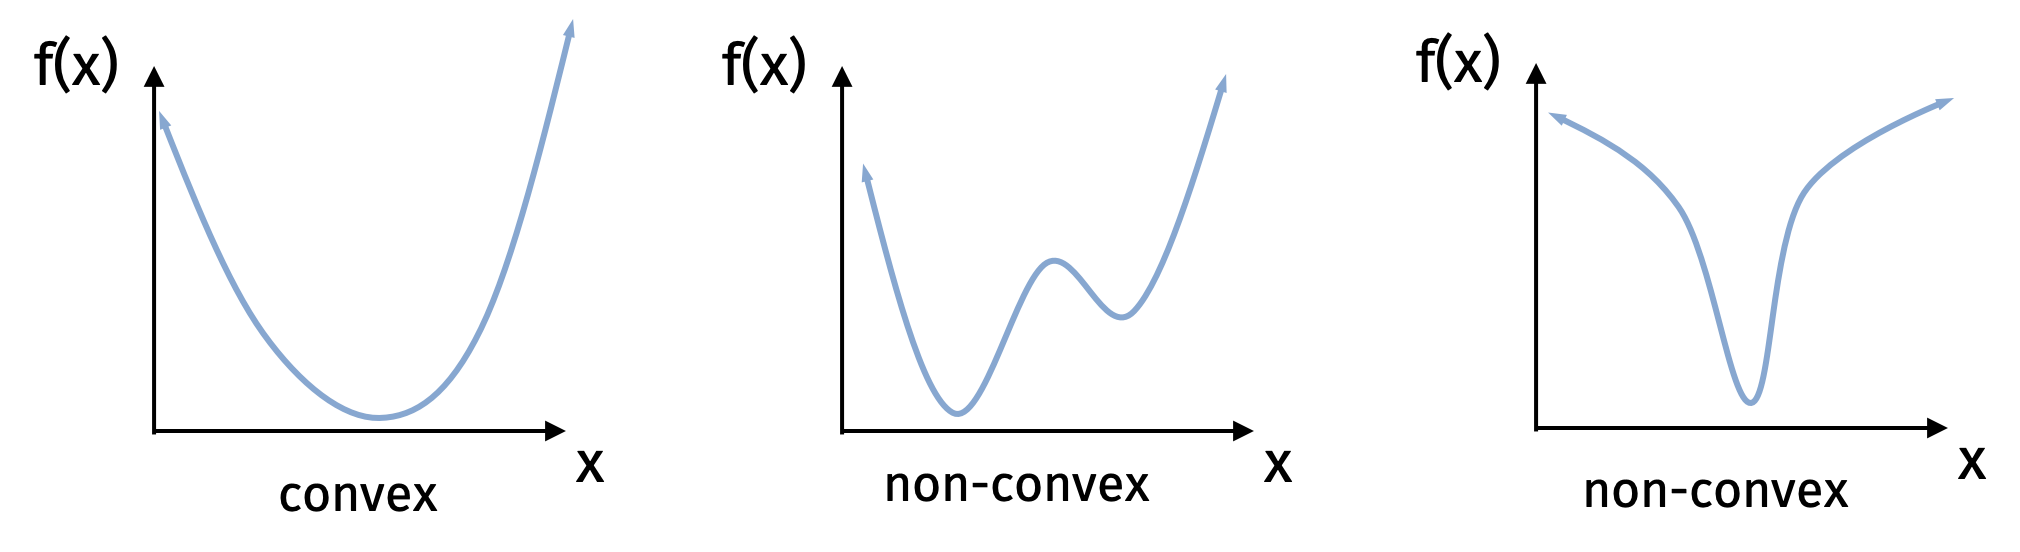
\includegraphics[width=\textwidth]{nonconvex_converge.png}
	\end{center}
	One issue with non-convex functions is that they can have \alert{\textbf{local minima}}. Even when they don't, convergence analysis requires different assumptions than convex functions. 	
\end{frame}

\begin{frame}[t]
	\frametitle{approach for this unit}
	We care about \emph{how fast} gradient descent and related methods converge, not just that they do converge. 
	\begin{itemize}
		\item Bounding iteration complexity requires placing some assumptions on $f(\bv{x})$. 
		\item Stronger assumptions lead to better bounds on the convergence. 
	\end{itemize}
	Understanding these assumptions can help us design faster variants of gradient descent (there are many!). 
	
	\begin{center}
		Today, we will start with \textbf{convex} functions. 
	\end{center}
\end{frame}

\begin{frame}[t]
	\frametitle{convexity}
	\begin{definition}[Convex]
		A function $f$ is convex iff for any $\bv{x}, \bv{y},\lambda \in [0,1]$:
		\begin{align*}
		(1-\lambda)\cdot f(\bv{x}) + \lambda \cdot f(\bv{y}) \geq f\left((1-\lambda)\cdot\bv{x} + \lambda \cdot\bv{y}\right)
		\end{align*}
	\end{definition}
\vspace{-.5em}
\begin{center}
	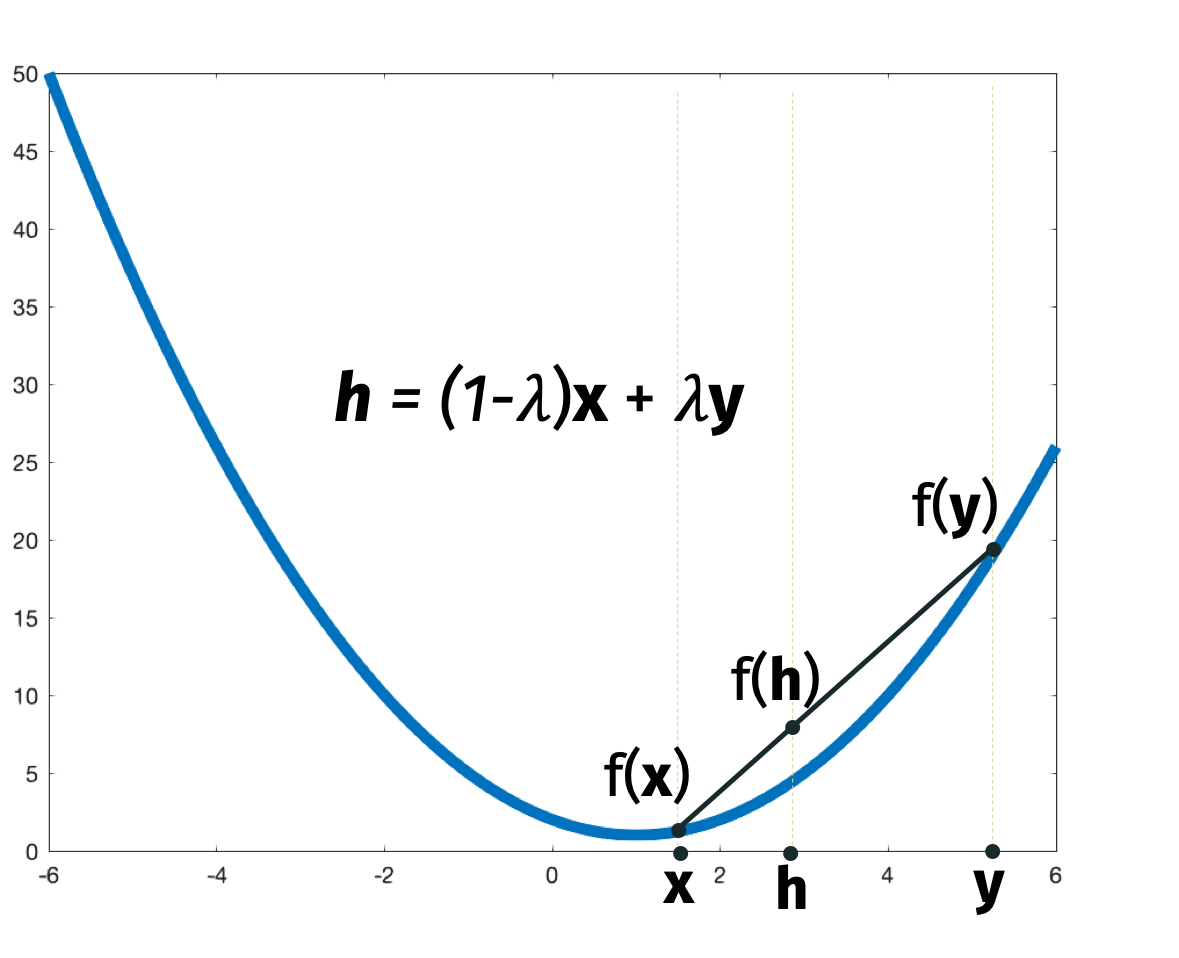
\includegraphics[width=.6\textwidth]{convex1.png}
\end{center}
\end{frame}


\begin{frame}[t]
	\frametitle{gradient descent}
	\small
		\begin{definition}[Convex]
		A function $f$ is convex if and only if for any $\bv{x}, \bv{y}$:
		\begin{align*}
			f(\bv{x} + \bv{z}) \geq f(\bv{x}) + \nabla f(\bv{x})^T\bv{z}
		\end{align*}
	\vspace{-1em}
	Equivalently:
	\vspace{-.5em}
		\begin{align*}
			f(\bv{x}) - f(\bv{y}) \leq \nabla f(\bv{x})^T (\bv{x} - \bv{y})
		\end{align*}
	\vspace{-1em}
	\end{definition}

	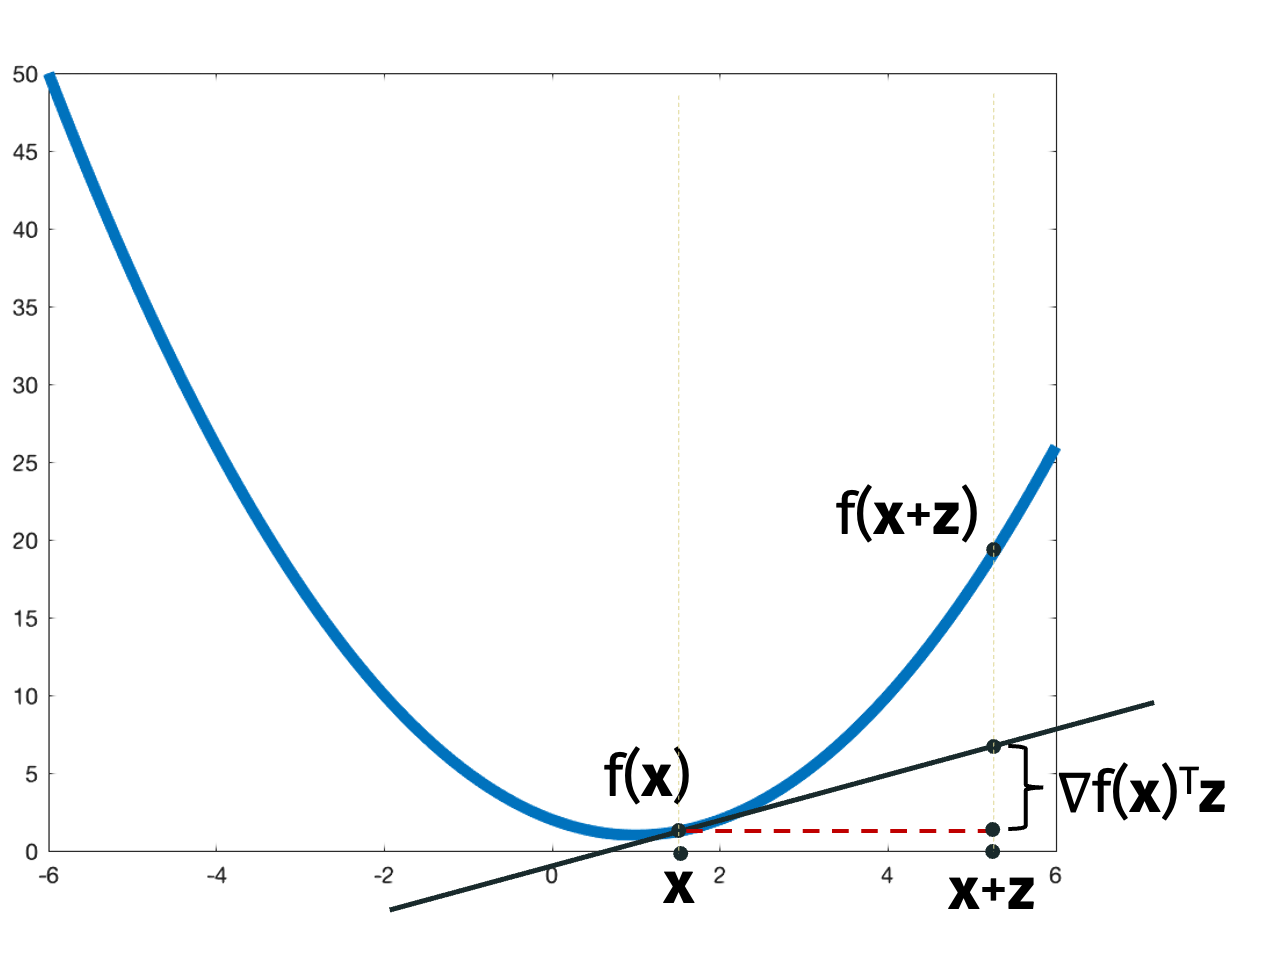
\includegraphics[width=.5\textwidth]{convex2.png}

\end{frame}

\begin{frame}
	\frametitle{definitions of convexity}
	It is easy but not obvious how to prove the equivalence between these definitions. A short proof can be found in Karthik Sridharan's lecture notes here:
	\begin{center}
		\color{blue}
		\href{http://www.cs.cornell.edu/courses/cs6783/2018fa/lec16-supplement.pdf}{http://www.cs.cornell.edu/courses/cs6783/2018fa/lec16-supplement.pdf}
	\end{center}
	
\end{frame}

\begin{frame}[t]
	\frametitle{gradient descent analysis}
	\textbf{Assume:}
	\begin{itemize}
		\item $f$ is convex.
		\item Lipschitz function: for all $\bv{x}$, $\|\nabla f(\bv{x})\|_2 \leq \alert{G}$.
		\item Starting radius: $\|\bv{x}^{*} - \bv{x}^{(0)}\|_2 \leq \alert{R}$.
	\end{itemize}
	
	\textbf{Gradient descent:}
	\begin{itemize}
		\item Choose number of steps $T$.
		\item Starting point $\bv{x}^{(0)}$. E.g.  $\bv{x}^{(0)} = \vec{0}$.
		\item $\eta = \frac{R}{G\sqrt{T}}$
		\item For $i = 0,\ldots, T$:
		\begin{itemize}
			\item $\bv{x}^{(i+1)} = \bv{x}^{(i)} - \eta \nabla f(\bv{x}^{(i)})$
		\end{itemize}
		\item Return $\hat{\bv{x}} = \argmin_{\bv{x}^{(i)}} f(\bv{x}^{(i)})$.
%		\item Alternatively, return $\hat{\bv{x}} = \frac{1}{T}\sum_{i=1}^T \bv{x}^{(i)}$.
	\end{itemize}
\end{frame}

\begin{frame}[t]
	\frametitle{gradient descent analysis}
	\begin{claim}[GD Convergence Bound]
		If we run GD for $T \geq \frac{R^2G^2}{\epsilon^2}$ iterations then $f(\hat{\bv{x}}) \leq f(\bv{x}^*) + \epsilon$.
	\end{claim}


	\vspace{12em}
	Proof is made tricky by the fact that $f(\bv{x}^{(i)})$ does not improve monotonically. We can ``overshoot" the minimum. 
\end{frame}

\begin{frame}[t]
	\frametitle{gradient descent analysis}
	\begin{claim}[GD Convergence Bound]
		If we run GD for $T \geq \frac{R^2G^2}{\epsilon^2}$ iterations with step-size $\eta = \frac{R}{G\sqrt{T}}$, then $f(\hat{\bv{x}}) \leq f(\bv{x}^*) + \epsilon$.
	\end{claim}

	Proof is made tricky by the fact that $f(\bv{x}^{(i)})$ does not improve monotonically. We can ``overshoot" the minimum. 
	
	We will prove that the \emph{average} solution value is low after $T = \frac{R^2G^2}{\epsilon^2}$ iterations. I.e. that:
	\begin{align*}
		\frac{1}{T}\sum_{i=0}^{T-1}\left[f(\bv{x}^{(i)}) - f(\bv{x}^*)\right]  \leq \epsilon.
	\end{align*}
Of course the best solution found, $\hat{\bv{x}}$ is only better than the average.
\end{frame}

\begin{frame}[t]
	\frametitle{gradient descent analysis}
	\small
	\begin{claim}[GD Convergence Bound]
		If we run GD for $T \geq \frac{R^2G^2}{\epsilon^2}$ iterations with step-size $\eta = \frac{R}{G\sqrt{T}}$, then $f(\hat{\bv{x}}) \leq f(\bv{x}^*) + \epsilon$.
	\end{claim}
	\textbf{Claim 1:} For all $i = 0, \ldots, T$, 
	\begin{align*}
		f(\bv{x}^{(i)}) - f(\bv{x}^*) \leq \frac{\|\bs{x}^{(i)} - \bs{x}^*\|_2^2 - \|\bs{x}^{(i+1)} -\bs{x}^*\|_2^2}{2\eta} + \frac{\eta G^2}{2}
	\end{align*}
	
	\textbf{Claim 1(a):} For all $i = 0, \ldots, T$, 
	\begin{align*}
		\nabla f(\bv{x}^{(i)})^T(\bs{x}^{(i)} - \bs{x}^{*})  \leq \frac{\|\bs{x}^{(i)} - \bs{x}^*\|_2^2 - \|\bs{x}^{(i+1)} -\bs{x}^*\|_2^2}{2\eta} + \frac{\eta G^2}{2}
	\end{align*}
	
	Claim 1 follows from Claim 1(a) by definition of convexity.
\end{frame}

\begin{frame}[t]
	\frametitle{gradient descent analysis}
	\small
	\begin{claim}[GD Convergence Bound]
		If we run GD for $T \geq \frac{R^2G^2}{\epsilon^2}$ iterations with step size $\eta = \frac{R}{G\sqrt{T}}$, then $f(\hat{\bv{x}}) \leq f(\bv{x}^*) + \epsilon$.
	\end{claim}
	\textbf{Claim 1(a):} For all $i = 0, \ldots, T$, 
	\begin{align*}
		 \frac{\|\bv{x}^{(i)} - \bv{x}^*\|_2^2 - \|\bv{x}^{(i+1)} -\bv{x}^*\|_2^2}{2\eta} + \frac{\eta G^2}{2} \geq \nabla f(\bv{x}^{(i)})^T(\bv{x}^{(i)} - \bv{x}^{*})
	\end{align*}
\end{frame}

%\begin{frame}[t]
%	\frametitle{gradient descent analysis}
%	\small
%	\begin{claim}[GD Convergence Bound]
%		If $T \geq \frac{R^2G^2}{\epsilon^2}$ and $\eta = \frac{R}{G\sqrt{T}}$, then $f(\hat{\bv{x}}) \leq f(\bv{x}^*) + \epsilon$.
%	\end{claim}
%	\textbf{Claim 1:} For all $i = 0, \ldots, T$, 
%	\begin{align*}
%		f(\bv{x}^{(i)}) - f(\bv{x}^*) \leq \frac{\|\bv{x}^{(i)} - \bv{x}^*\|_2^2 - \|\bv{x}^{(i+1)} - \bv{x}^*\|_2^2}{2\eta} + \frac{\eta G^2}{2}
%	\end{align*}
%	\textbf{Telescoping sum:}
%	\begin{align*}
%		\sum_{i=0}^{T-1}\left[f(\bv{x}^{(i)}) - f(\bv{x}^*)\right] &\leq \frac{\|\bv{x}^{(0)} - \bv{x}^*\|_2^2 - \|\bv{x}^{(T)} - \bv{x}^*\|_2^2}{2\eta} + \frac{T\eta G^2}{2}\\
%		\frac{1}{T}\sum_{i=0}^{T-1}\left[f(\bv{x}^{(i)}) - f(\bv{x}^*)\right] &\leq \frac{R^2}{2T\eta} + \frac{\eta G^2}{2}
%	\end{align*}
%\end{frame}
%
%\begin{frame}[t]
%	\frametitle{gradient descent analysis}
%	\small
%	\textbf{Telescoping sum:}
%	\begin{align*}
%		\sum_{i=0}^{T-1}\left[f(\bv{x}^{(i)}) - f(\bv{x}^*)\right] &\leq \frac{\|\bv{x}^{(0)} - \bv{x}^*\|_2^2 - \|\bv{x}^{(T)} - \bv{x}^*\|_2^2}{2\eta} + \frac{T\eta G^2}{2}\\
%		\frac{1}{T}\sum_{i=0}^{T-1}\left[f(\bv{x}^{(i)}) - f(\bv{x}^*)\right] &\leq \frac{R^2}{2T\eta} + \frac{\eta G^2}{2}
%	\end{align*}
%\end{frame}
%
%\begin{frame}[t]
%	\frametitle{gradient descent analysis}
%	\begin{claim}[GD Convergence Bound]
%		If $T \geq \frac{R^2G^2}{\epsilon^2}$ and $\eta = \frac{R}{G\sqrt{T}}$, then $f(\hat{\bv{x}}) \leq f(\bv{x}^*) + \epsilon$.
%	\end{claim}
%	\textbf{Final step:}
%	\begin{align*}
%		\frac{1}{T}\sum_{i=0}^{T-1}\left[f(\bv{x}^{(i)}) - f(\bv{x}^*)\right] &\leq \epsilon \\ 
%		\left[\frac{1}{T}\sum_{i=0}^{T-1}f(\bv{x}^{(i)})\right] - f(\bv{x}^*) &\leq \epsilon 
%	\end{align*}
%	We always have that $\min_i f(\bv{x}^{(i)}) \leq \frac{1}{T}\sum_{i=0}^{T-1}f(\bv{x}^{(i)})$, so this is what we return:
%	\begin{align*}
%		L(\hat{\bv{x}}) = \min_{i\in 1,\ldots, T} f(\bv{x}^{(i)}) \leq f(\bv{x}^*) + \epsilon. 
%	\end{align*}
%\end{frame}

%\begin{frame}[t]
%	\frametitle{gradient descent analysis}
%	\begin{claim}[GD Convergence Bound]
%		If $T \geq \frac{R^2G^2}{\epsilon^2}$ and $\eta = \frac{R}{G\sqrt{T}}$, then $f(\hat{\bv{x}}) \leq f(\bv{x}^*) + \epsilon$.
%	\end{claim}
%\textbf{Claim 1:} For all $i = 0, \ldots, T$, 
%\begin{align*}
%	f(\bv{x}^{(i)}) - f(\bv{x}^*) \leq \frac{\|\bv{x}^{(i)} - \bv{x}^*\|_2^2 - \|\bv{x}^{(i+1)} - \bv{x}^*\|_2^2}{2\eta} + \frac{\eta G^2}{2}
%\end{align*}
%
%\end{frame}

\begin{frame}[t]
	\frametitle{gradient descent analysis}
	\footnotesize
	\begin{claim}[GD Convergence Bound]
		If $T \geq \frac{R^2G^2}{\epsilon^2}$ and $\eta = \frac{R}{G\sqrt{T}}$, then $f(\bv{\hat{x}}) \leq f(\bv{x}^*) + \epsilon$.
	\end{claim}
	\textbf{Claim 1:} For all $i = 0, \ldots, T$, 
	\begin{align*}
		f(\bv{x}^{(i)}) - f(\bv{x}^*) \leq \frac{\|\bv{x}^{(i)} - \bv{x}^*\|_2^2 - \|\bv{x}^{(i+1)} - \bv{x}^*\|_2^2}{2\eta} + \frac{\eta G^2}{2}
	\end{align*}
	\textbf{Telescoping sum:}
	\begin{align*}
		\sum_{i=0}^{T-1}\left[f(\bv{x}^{(i)}) - f(\bv{x}^*)\right] &\leq \frac{\|\bv{x}^{(0)} - \bv{x}^*\|_2^2 - \|\bv{x}^{(1)} - \bv{x}^*\|_2^2}{2\eta} + \frac{\eta G^2}{2}\\
		&+ \frac{\|\bv{x}^{(1)} - \bv{x}^*\|_2^2 - \|\bv{x}^{(2)} - \bv{x}^*\|_2^2}{2\eta} + \frac{\eta G^2}{2}\\
		&+ \frac{\|\bv{x}^{(2)} - \bv{x}^*\|_2^2 - \|\bv{x}^{(3)} - \bv{x}^*\|_2^2}{2\eta} + \frac{\eta G^2}{2}\\
		&\vdots\\
		&+ \frac{\|\bv{x}^{(T-1)} - \bv{x}^*\|_2^2 - \|\bv{x}^{(T)} - \bv{x}^*\|_2^2}{2\eta} + \frac{\eta G^2}{2}
	\end{align*}
	
	\begin{align*}
		\sum_{i=0}^{T-1}\left[f(\bv{x}^{(i)}) - f(\bv{x}^*)\right] &\leq \frac{\|\bv{x}^{(0)} - \bv{x}^*\|_2^2 - \|\bv{x}^{(T)} - \bv{x}^*\|_2^2}{2\eta} + \frac{T\eta G^2}{2}\\
		\frac{1}{T}\sum_{i=0}^{T-1}\left[f(\bv{x}^{(i)}) - f(\bv{x}^*)\right] &\leq \frac{R^2}{2T\eta} + \frac{\eta G^2}{2}
	\end{align*}
\end{frame}

\begin{frame}[t]
	\frametitle{gradient descent analysis}
	\small
	\begin{claim}[GD Convergence Bound]
	If $T \geq \frac{R^2G^2}{\epsilon^2}$ and $\eta = \frac{R}{G\sqrt{T}}$, then $f(\hat{\bv{x}}) \leq f(\bv{x}^*) + \epsilon$.
	\end{claim}
\textbf{Telescoping sum:}
\begin{align*}
	\sum_{i=0}^{T-1}\left[f(\bv{x}^{(i)}) - f(\bv{x}^*)\right] &\leq \frac{\|\bv{x}^{(0)} - \bv{x}^*\|_2^2 - \|\bv{x}^{(T)} - \bv{x}^*\|_2^2}{2\eta} + \frac{T\eta G^2}{2}\\
	\frac{1}{T}\sum_{i=0}^{T-1}\left[f(\bv{x}^{(i)}) - f(\bv{x}^*)\right] &\leq \frac{R^2}{2T\eta} + \frac{\eta G^2}{2}
\end{align*}
\end{frame}
\begin{frame}[t]
	\frametitle{gradient descent analysis}
	\begin{claim}[GD Convergence Bound]
		If $T \geq \frac{R^2G^2}{\epsilon^2}$ and $\eta = \frac{R}{G\sqrt{T}}$, then $f(\hat{\bv{x}}) \leq f(\bv{x}^*) + \epsilon$.
	\end{claim}
	\textbf{Final step:}
	\begin{align*}
		\frac{1}{T}\sum_{i=0}^{T-1}\left[f(\bv{x}^{(i)}) - f(\bv{x}^*)\right] &\leq \epsilon \\ 
		\left[\frac{1}{T}\sum_{i=0}^{T-1}f(\bv{x}^{(i)})\right] - f(\bv{x}^*) &\leq \epsilon 
	\end{align*}
We always have that $f(\hat{\bv{x}}) = \min_i f(\bv{x}^{(i)}) \leq \frac{1}{T}\sum_{i=0}^{T-1}f(\bv{x}^{(i)})$, which gives the final bound:
\begin{align*}
	f(\hat{\bv{x}}) \leq f(\bv{x}^*) + \epsilon. 
\end{align*}
\end{frame}

\begin{frame}[t]
	\frametitle{constrained convex optimization}
	\textbf{Typical goal}: Solve a \emph{convex minimization problem} with additional \emph{convex constraints}.  
	\begin{align*}
		\min_{\bv{x}\in \mathcal{S}} f(\bv{x})
	\end{align*}
where $\mathcal{S}$ is a \textbf{\alert{convex set}}. 
\begin{center}
	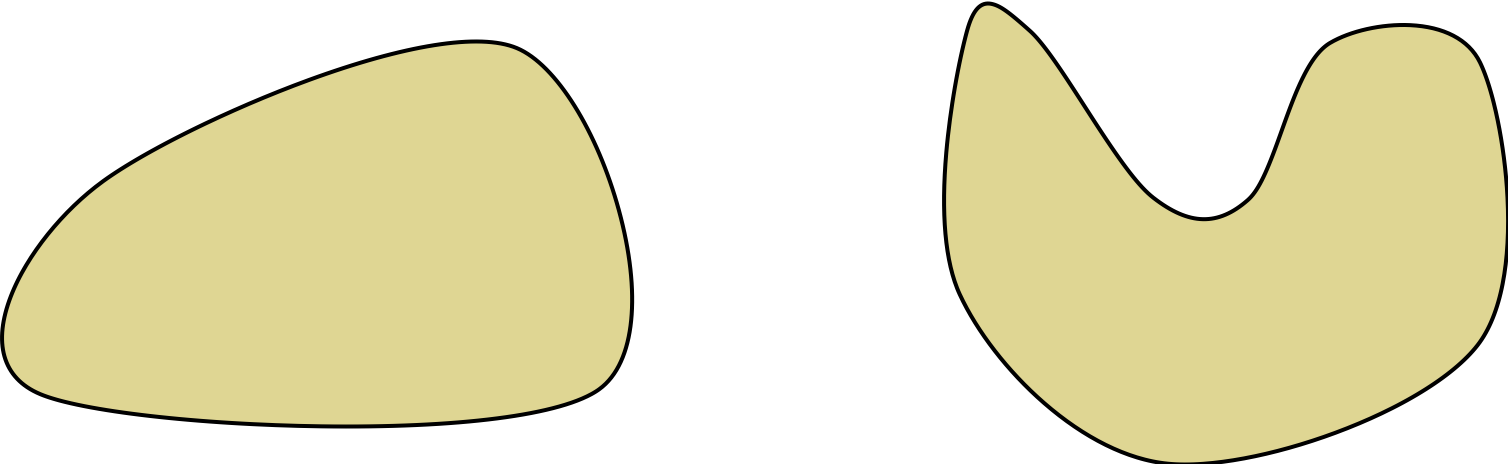
\includegraphics[width=.7\textwidth]{sets.png}
	
	Which of these is convex?
\end{center}
\end{frame}

\begin{frame}[t]
	\frametitle{constrained convex optimization}
	\begin{center}
		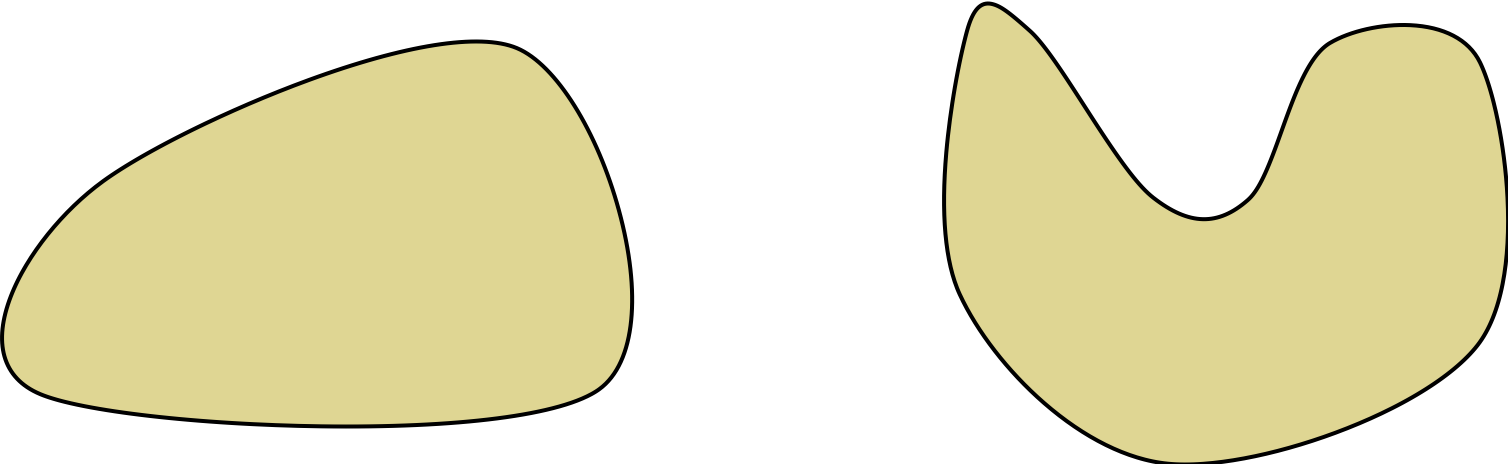
\includegraphics[width=.7\textwidth]{sets.png}
	\end{center}

	\begin{definition}[Convex set]
		A set $\mathcal{S}$ is convex if for any $\bv{x}, \bv{y} \in \mathcal{S}, \lambda \in [0,1]$:
		\begin{align*}
			(1-\lambda)\bv{x} + \lambda\bv{y} \in \mathcal{S}.
		\end{align*}
	\end{definition}
\end{frame}

\begin{frame}[t]
	\frametitle{constrained convex optimization}
	\textbf{Examples:}
	\begin{itemize}
		\item \textbf{Norm constraint:} minimize $\|\bv{A}\bv{x} - \bv{b}\|_2$ subject to $\|\bv{x}\|_2 \leq \lambda$. Used e.g. for regularization, finding a sparse solution, etc.
		\item \textbf{Positivity constraint:} minimize $f(\bv{x})$ subject to $\bv{x} \geq 0$. 
		% Used e.g. in finding an optimal allocation for a portfolio into different assets. 
		\item \textbf{Linear constraint:} minimize $\bv{c}^T\bv{x}$ subject to $\bv{A}\bv{x} \leq \bv{b}$. Linear program used in training support vector machines, industrial optimization, subroutine in integer programming, etc.
	\end{itemize}
\end{frame}

\begin{frame}[t]
	\frametitle{problem with gradient descent}
	\textbf{Gradient descent:}
	\begin{itemize}
		\item For $i = 0,\ldots, T$:
		\begin{itemize}
			\item $\bv{x}^{(i+1)} = \bv{x}^{(i)} - \eta \nabla f(\bv{x}^{(i)})$
		\end{itemize}
		\item Return $\hat{\bv{x}} = \argmin_{i} f(\bv{x}^{(i)})$.
	\end{itemize}
	
	\begin{center}
		\alert{
		Even if we start with $\bv{x}^{(0)} \in \mathcal{S}$, there is no guarantee that $ \bv{x}^{(0)} - \eta \nabla f(\bv{x}^{(0)})$ will remain in our set.}
	\end{center}

	\textbf{Extremely simple modification:} Force $\bv{x}^{(i)}$ to be in $\mathcal{S}$ by \textbf{\alert{projecting}} onto the set.
\end{frame}

\begin{frame}
	\frametitle{constrained first order optimization}
	Given a function $f$ to minimize and a convex constraint set $\mathcal{S}$, assume we have:
	\begin{itemize}
		\item \textbf{Function oracle}: Evaluate $f(\bv{x})$ for any $\bv{x}$. 
		\item \textbf{Gradient oracle}: Evaluate $\nabla f(\bv{x})$ for any $\bv{x}$.
		\item \textbf{\alert{Projection oracle}}: Evaluate $P_{\mathcal{S}}(\bv{x})$ for any $\bv{x}$.
	\end{itemize}
\begin{align*}
	P_{\mathcal{S}}(\bv{x}) = \argmin_{\bv{y}\in \mathcal{S}} \|\bv{x} - \bv{y}\|_2
\end{align*}
\end{frame}

\begin{frame}
	\frametitle{projection oracles}
	\begin{itemize}
		\item How would you implement $P_\mathcal{S}$ for $\mathcal{S} = \{\bv{y}:\|\bv{y}\|_2\leq 1\}.$
		\item How would you implement $P_\mathcal{S}$ for $\mathcal{S} = \{\bv{y}:\bv{y} = \bv{Q}\bv{z}\}.$
	\end{itemize}
\begin{center}
	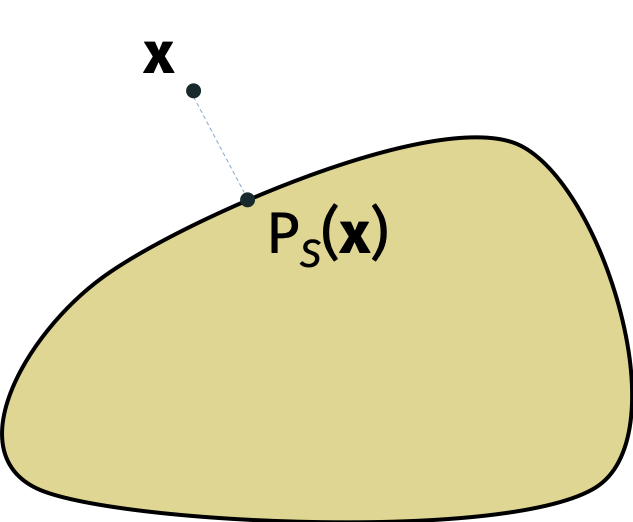
\includegraphics[width=.5\textwidth]{projection_image.png}
\end{center}
\end{frame}

\begin{frame}[t]
	\frametitle{projected gradient descent}
	Given function $f(\bv{x})$ and set $\mathcal{S}$, such that $\|\nabla f(\bv{x})\|_2 \leq G$ for all $\bv{x}\in \mathcal{S}$ and starting point $\bv{x}^{(0)}$ with $\|\bv{x}^{(0)} - \bv{x}^*\|_2 \leq R$.  
	
	\textbf{Projected gradient descent:}
	\begin{itemize}
		\item Select starting point $\bv{x}^{(0)}$, $\eta = \frac{R}{G\sqrt{T}}$. 
		\item For $i = 0,\ldots, T$:
		\begin{itemize}
			\item $\bv{z} = \bv{x}^{(i)} - \eta \nabla f(\bv{x}^{(i)})$
			\item $\bv{x}^{(i+1)} = P_\mathcal{S}(\bv{z})$
		\end{itemize}
		\item Return $\hat{\bv{x}} = \argmin_{i} f(\bv{x}^{(i)})$.
	\end{itemize}
\begin{claim}[PGD Convergence Bound]
	If $f, \mathcal{S}$ are convex and $T \geq \frac{R^2G^2}{\epsilon^2}$, then $f(\hat{\bv{x}}) \leq f(\bv{x}^*) + \epsilon$.
\end{claim}
\end{frame}

\begin{frame}[t]
	\frametitle{projected gradient descent analysis}
	Analysis is almost identical to standard gradient descent! We just need one additional claim:
	
	\begin{claim}[Contraction Property of Convex Projection]
		If $\mathcal{S}$ is convex, then for \emph{any} $\bv{y} \in \mathcal{S}$,
		\begin{align*}
			\|\bv{y} - P_\mathcal{S}(\bv{x})\|_2 \leq \|\bv{y} - \bv{x}\|_2.
		\end{align*}
	\end{claim}
\vspace{-1em}
\begin{center}
	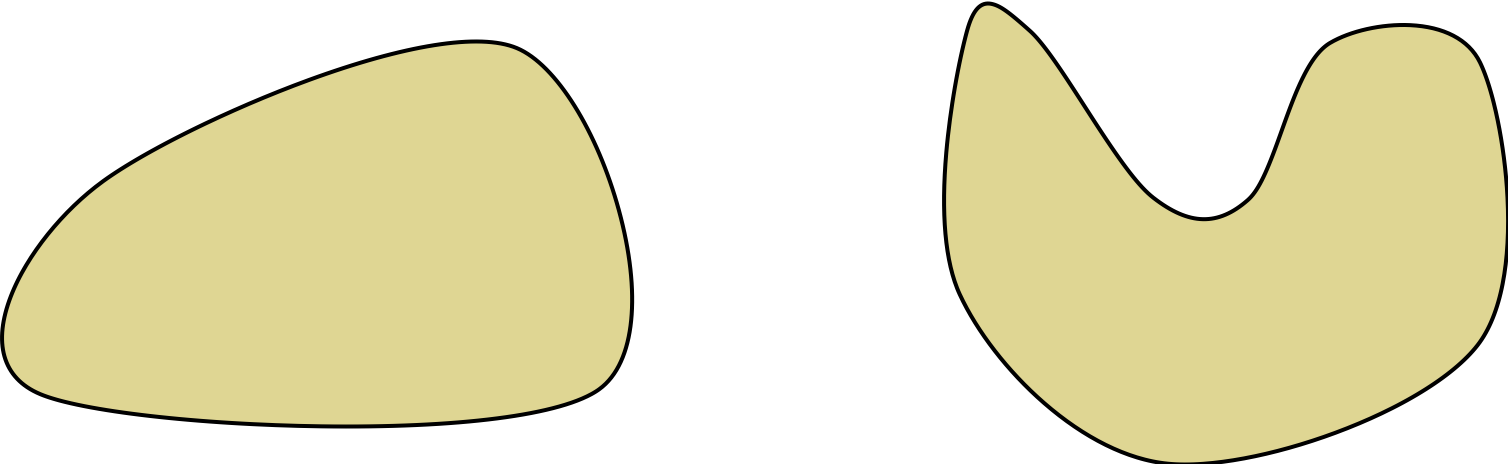
\includegraphics[width=.8\textwidth]{sets.png}
\end{center}	
\end{frame}

\begin{frame}[t]
	\frametitle{gradient descent analysis}
	\small
\begin{claim}[PGD Convergence Bound]
	If $f, \mathcal{S}$ are convex and $T \geq \frac{R^2G^2}{\epsilon^2}$, then $f(\hat{\bv{x}}) \leq f(\bv{x}^*) + \epsilon$.
\end{claim}
	\textbf{Claim 1:} For all $i = 0, \ldots, T$, let $\bv{z}^{(i)} = \bv{x}^{(i)} - \eta \nabla f(\bv{x}^{(i)})$. Then:
	\begin{align*}
		f(\bv{x}^{(i)}) - f(\bv{x}^*) &\leq \frac{\|\bv{x}^{(i)} - \bv{x}^*\|_2^2 - \|\bv{z}^{(i)} - \bv{x}^*\|_2^2}{2\eta} + \frac{\eta G^2}{2}
		\\&\leq \frac{\|\bv{x}^{(i)} - \bv{x}^*\|_2^2 - \|\bv{x}^{(i+1)} - \bv{x}^*\|_2^2}{2\eta} + \frac{\eta G^2}{2}
	\end{align*}
\vspace{4em}

\textbf{Same telescoping sum argument:}\vspace{-.5em}
\begin{align*}
	\left[\frac{1}{T}\sum_{i=0}^{T-1}f(\bv{x}^{(i)})\right] - f(\bv{x}^*) \leq \frac{R^2}{2T\eta} + \frac{\eta G^2}{2}.
\end{align*}
\end{frame}

\begin{frame}[t]
	\frametitle{gradient descent}
	\textbf{Conditions:}
	\begin{itemize}
		\item \textbf{Convexity:} $f$ is a convex function, $\mathcal{S}$ is a convex set. 
		\item \textbf{Bounded initial distant:} 
		\begin{align*}
			\|\bv{x}^{(0)} - \bv{x}^*\|_2 \leq \alert{R}
		\end{align*}
		\item \textbf{Bounded gradients (Lipschitz function)}: 
		\begin{align*}
			\|\nabla f(\bv{x})\|_2 \leq \alert{G} \text{ for all } \bv{x}\in \mathcal{S}.
		\end{align*}
	\end{itemize}
	
	\begin{theorem}[GD Convergence Bound]
		(Projected) Gradient Descent returns $\hat{\bv{x}}$ with $f(\hat{\bv{x}}) \leq \min_{\bv{x}\in \mathcal{S}}f(\bv{x})+\epsilon$ after
		\begin{align*}
			T = \frac{R^2 G^2}{\epsilon^2} \text{ iterations.}
		\end{align*}
	\end{theorem}
\end{frame}

\begin{frame}
	\frametitle{beyond the basic bound}
	Can our convergence bound be tightened for certain functions? Can it guide us towards faster algorithms?
	
	\textbf{Goals:}
	\begin{itemize}
		\item Improve $\epsilon$ dependence below $1/\epsilon^2$.
		\begin{itemize}
			\item Ideally $1/\epsilon$ or $\log(1/\epsilon)$. 
		\end{itemize}
		\item Reduce or eliminate dependence on $G$ and $R$.
	\end{itemize}
	\alert{\textbf{Will need to take advantage of additional problem structure.}}
\end{frame}

\begin{frame}[t]
	\frametitle{smoothness}
	\begin{definition}[$\beta$-smoothness]
		A function $f$ is $\alert{\beta}$ smooth if, for all $\bv{x}$, $\bv{y}$
		\begin{align*}
			\|\nabla f(\bv{x}) - \nabla f(\bv{y})\|_2 \leq \alert{\beta} \|\bv{x} - \bv{y}\|_2
		\end{align*}
	\end{definition}
	For a scalar valued function $f$, equivalent to $f''(x) \leq \beta$. 
	\vspace{4em}
	After some calculus (see Lem. 3.4 in \color{blue}\textbf{\href{https://arxiv.org/pdf/1405.4980.pdf}{Bubeck's book}}\color{black}), this implies:
	\begin{align*}
		\left[f(\bv{y}) - f(\bv{x})\right] - \nabla f(\bv{x})^T(\bv{y} - \bv{x})  \leq \frac{\beta}{2}\|\bv{x} - \bv{y}\|_2^2
	\end{align*}
\end{frame}

\begin{frame}[t]
	\frametitle{smoothness}
	Recall from convexity that $f(\bv{y}) - f(\bv{x}) \geq \nabla f(\bv{x})^T(\bv{y} - \bv{x})$.
	\begin{center}
		\alert{So now we have an upper and lower bound.}
	\end{center}
\vspace{-1em}
	\begin{align*}
		0 \leq \left[f(\bv{y}) - f(\bv{x})\right] - \nabla f(\bv{x})^T(\bv{y} - \bv{x}) \leq \frac{\beta}{2}\|\bv{x} - \bv{y}\|_2^2
	\end{align*}
\vspace{-2em}
\begin{center}
	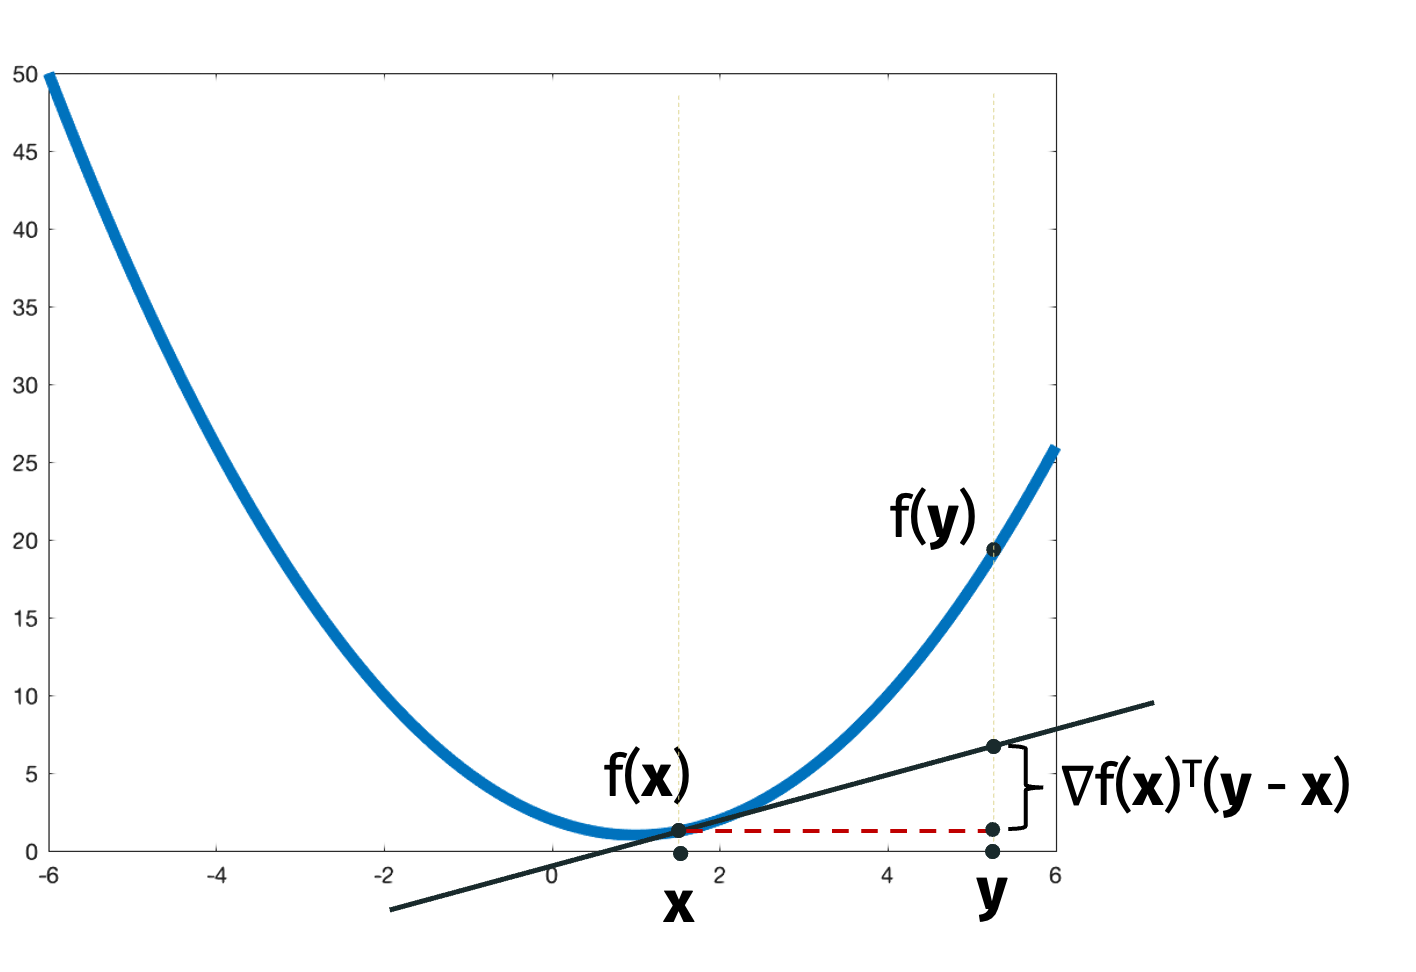
\includegraphics[width=.75\textwidth]{smoothness_image.png}
\end{center}	
\end{frame}

\begin{frame}[t]
	\frametitle{convergence guarantee}
	\begin{theorem}[GD convergence for $\beta$-smooth functions.]
		Let $f$ be a \alert{$\beta$} smooth convex function and assume we have $\|\bv{x}^{*} - \bv{x}^{(1)}\|_2 \leq \alert{R}$. If we run GD for $T$ steps, we have:
		\begin{align*}
			f(\bv{x}^{(T)}) - f(\bv{x}^*) \leq \frac{2\beta R^2}{T} 
		\end{align*} 
	\end{theorem}
	\textbf{Corollary}: If \alert{$T = O\left(\frac{\beta R^2}{\epsilon}\right)$} we have $f(\bv{x}^{(T)}) - f(\bv{x}^*) \leq \epsilon$.
	
	\vspace{1em}
		Compare this to $T = O\left(\frac{G^2 R^2}{\epsilon^2}\right)$ without  a smoothness assumption.
\end{frame}

\begin{frame}[t]
	\frametitle{guaranteed progress}
	\begin{center}
	Why do you think gradient descent might be faster when a function is $\beta$-smooth? Think about scalar case, in which case smoothness means $f''(x) \leq \beta$. 
	\end{center}
\end{frame}

\begin{frame}[t]
	\frametitle{guaranteed progress}
	Previously learning rate/step size $\eta$ depended on $G$. Now choose it based on $\beta$:
	\begin{align*}
		\bv{x}^{(t+1)} \leftarrow \bv{x}^{(t)} - \frac{1}{\beta}\nabla f(\bv{x}^{(t)})
	\end{align*}
	
	\textbf{Progress per step of gradient descent:}
	\begin{enumerate}[1.]
		\item $\left[f(\bv{x}^{(t+1)}) - f(\bv{x}^{(t)})\right] - \nabla f(\bv{x}^{(t)})^T(\bv{x}^{(t+1)} - \bv{x}^{(t)})  \leq \frac{\beta}{2}\|\bv{x}^{(t)} - \bv{x}^{(t+1)}\|_2^2.$\vspace{1.5em}
		\item $\left[f(\bv{x}^{(t+1)}) - f(\bv{x}^{(t)})\right] + 
		\frac{1}{\beta}\|\nabla f(\bv{x}^{(t)})\|_2^2 \leq \frac{\beta}{2}\|\frac{1}{\beta}\nabla f(\bv{x}^{(t)})\|_2^2.$\vspace{1.5em}
		\item $f(\bv{x}^{(t)}) - f(\bv{x}^{(t+1)}) \geq \alert{\frac{1}{2\beta}\|\nabla f(\bv{x}^{(t)})\|_2^2}.$
	\end{enumerate}
%	\begin{align*}
%		\left[f(\bv{x}^{(t+1)}) - f(\bv{x}^{(t)})\right] - \nabla f(\bv{x}^{(t)})^T(\bv{x}^{(t+1)} - \bv{x}^{(t)})  \leq \frac{\beta}{2}\|\bv{x}^{(t)} - \bv{x}^{(t+1)}\|_2^2\\
%	\end{align*}
%	\begin{align*}
%		\left[f(\bv{x}^{(t+1)}) - f(\bv{x}^{(t)})\right] + 
%		\frac{1}{\beta}\|\nabla f(\bv{x}^{(t)})\|_2^2 \leq \frac{\beta}{2}\|\frac{1}{\beta}\nabla f(\bv{x}^{(t)})\|_2^2 \\
%	\end{align*}
%	\begin{align*}
%		f(\bv{x}^{(t)}) - f(\bv{x}^{(t+1)}) \geq \alert{\frac{1}{2\beta}\|\nabla f(\bv{x}^{(t)})\|_2^2}.
%	\end{align*}
\end{frame}

%\begin{frame}[t]
%	\frametitle{telescoping sum}
%	\textbf{Claim:} For all $t$, $f(\bv{x}^{(t)}) - f(\bv{x}^{(t+1)}) \geq \alert{\frac{1}{2\beta}\|\nabla f(\bv{x}^{(t)})\|_2^2}.$
%	
%	\begin{align*}
%		f(x^{(0)}) - f(x^{(T)}) \geq \frac{1}{2\beta} \sum_{t=0}^T\|\nabla f(\bv{x}^{(t)})\|_2^2
%	\end{align*}
%	
%\end{frame}


\begin{frame}[t]
	\frametitle{convergence guarantee}
	\begin{theorem}[GD convergence for $\beta$-smooth functions.]
		Let $f$ be a \alert{$\beta$} smooth convex function and assume we have $\|\bv{x}^{*} - \bv{x}^{(1)}\|_2 \leq \alert{R}$. If we run GD for $T$ steps with $\eta = \frac{1}{\beta}$ we have:
		\begin{align*}
			f(\bv{x}^{(T)}) - f(\bv{x}^*) \leq \frac{2\beta R^2}{T} 
		\end{align*} 
	\end{theorem}
	\textbf{Corollary}: If \alert{$T = O\left(\frac{\beta R^2}{\epsilon}\right)$} we have $f(\bv{x}^{(T)}) - f(\bv{x}^*) \leq \epsilon$.
	
	Again getting this result from the previous page is not hard, but also not obvious/direct. A concise proof can be found in \color{blue} \href{https://gowerrobert.github.io/pdf/M2_statistique_optimisation/grad_conv.pdf}{Garrigos and Gower's notes}.
\end{frame}

\begin{frame}[t]
	\frametitle{guaranteed progress}
	\begin{center}
		Where did we use convexity in this proof?
	\end{center}
	
	\textbf{Progress per step of gradient descent:}
	\begin{enumerate}[1.]
		\item $\left[f(\bv{x}^{(t+1)}) - f(\bv{x}^{(t)})\right] - \nabla f(\bv{x}^{(t)})^T(\bv{x}^{(t+1)} - \bv{x}^{(t)})  \leq \frac{\beta}{2}\|\bv{x}^{(t)} - \bv{x}^{(t+1)}\|_2^2.$\vspace{1.5em}
		\item $\left[f(\bv{x}^{(t+1)}) - f(\bv{x}^{(t)})\right] + 
		\frac{1}{\beta}\|\nabla f(\bv{x}^{(t)})\|_2^2 \leq \frac{\beta}{2}\|\frac{1}{\beta}\nabla f(\bv{x}^{(t)})\|_2^2.$\vspace{1.5em}
		\item $f(\bv{x}^{(t)}) - f(\bv{x}^{(t+1)}) \geq \alert{\frac{1}{2\beta}\|\nabla f(\bv{x}^{(t)})\|_2^2}.$
	\end{enumerate}
\end{frame}

\begin{frame}[t]
	\frametitle{stationary points}
	\begin{definition}[Stationary point]
		For a differentiable function $f$, a \emph{stationary point} is any $\bv{x}$ with: 
		\begin{align*}
			\nabla f(\bv{x}) = \bv{0}
		\end{align*}
	\end{definition}
	\begin{center}
		local/global minima - local/global maxima - saddle points
	\end{center}
\end{frame}

\begin{frame}[t]
	\frametitle{convergence to stationary point}
	\begin{theorem}[Convergence to Stationary Point]
	For \emph{any} $\beta$-smooth differentiable function $f$ (convex or not), if we run GD for $T$ steps, we can find a point $\hat{\bv{x}}$ such that:
	\begin{align*}
		\|\nabla f(\hat{\bv{x}})\|_2^2 \leq  \frac{2\beta}{T} \left( f(\bv{x}^{(0)}) -  f(\bv{x}^{*})\right)
	\end{align*} 
\end{theorem}
\textbf{Corollary:} If $T \geq \frac{2\beta}{\epsilon}$, then $\|\nabla f(\hat{\bv{x}})\|_2^2 \leq \epsilon  \left( f(\bv{x}^{(0)}) -  f(\bv{x}^{*})\right)$.
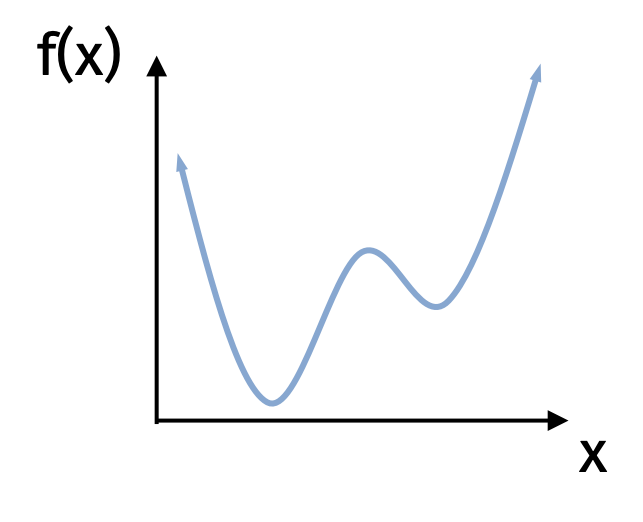
\includegraphics[width=.4\textwidth]{simple_non_convex.png}
\end{frame}

\begin{frame}[t]
	\frametitle{telescoping sum proof}
	\begin{theorem}[Convergence to Stationary Point]
		For \emph{any} $\beta$-smooth differentiable function $f$ (convex or not), if we run GD for $T$ steps, we can find a point $\hat{\bv{x}}$ such that:
		\begin{align*}
			\|\nabla f(\hat{\bv{x}})\|_2^2 \leq  \frac{2\beta}{T} \left( f(\bv{x}^{(0)}) -  f(\bv{x}^{*})\right) 
		\end{align*} 
	\end{theorem}
We have that $\frac{1}{2\beta}\|\nabla f(\bv{x}^{(t)})\|_2^2 \leq f(\bv{x}^{(t)}) - f(\bv{x}^{(t+1)}).$ So: 
\begin{align*}
	\sum_{t=0}^{T-1}\frac{1}{2\beta}\|\nabla f(\bv{x}^{(t)})\|_2^2 &\leq f(\bv{x}^{(0)}) -  f(\bv{x}^{(t)})\\
	\frac{1}{T}\sum_{t=0}^{T-1}\|\nabla f(\bv{x}^{(t)})\|_2^2 &\leq \frac{2\beta}{T} \left( f(\bv{x}^{(0)}) -  f(\bv{x}^{*})\right)\\
	\min_t \|\nabla f(\bv{x}^{(t)})\|_2^2 &\leq \frac{2\beta}{T} \left( f(\bv{x}^{(0)}) -  f(\bv{x}^{*})\right)
\end{align*}
\end{frame}

\begin{frame}[t]
	\frametitle{questions in non-convex optimization}
	\textbf{If GD can find a stationary point, are there algorithms which find a stationary point faster using preconditioning, acceleration, stochastic methods, etc.?}
\end{frame}

\begin{frame}[t]
	\frametitle{questions in non-convex optimization}
	\textbf{What if my function only has global minima and saddle points?}
	Randomized methods (SGD, perturbed gradient methods, etc.) can provably ``escape'' saddle points.
	\vspace{1em}
	
	
	\textbf{Example:} $\min_{\bv{x}} \frac{-\bv{x}^T\bv{A}^T\bv{A}\bv{x}}{\bv{x}^T\bv{x}}$
	\begin{itemize}
		\item \textbf{Global minimum}: Top eigenvector of $\bv{A}^T\bv{A}$ (i.e., top principal component of $\bv{A}$).
		\item \textbf{Saddle points:} All other eigenvectors of $\bv{A}$. 
	\end{itemize}
	\begin{center}
		\alert{\textbf{Useful for lots of other matrix factorization problems beyond vanilla PCA.}}
	\end{center}
\end{frame}

\begin{frame}[t]
	\frametitle{back to convex functions}
	I said it was a bit tricky to prove that $f(\hat{\bv{x}}) - f(\bv{x}^*) \leq \frac{2\beta R^2}{T}$ for convex functions. But we just easily proved that $\|\nabla f(\hat{\bv{x}})\|_2^2$ is small. Why doesn't this show we are close to the minimum?
	
\end{frame}

\begin{frame}[t]
	\frametitle{strong convexity}
	\begin{definition}[$\alpha$-strongly convex]
		A convex function $f$ is $\alert{\alpha}$-strongly convex if, for all $\bv{x}$, $\bv{y}$
		\begin{align*}
			\left[f(\bv{y}) - f(\bv{x})\right] - \nabla f(\bv{x})^T(\bv{y} - \bv{x}) \geq \frac{\alpha}{2}\|\bv{x} - \bv{y}\|_2^2 
		\end{align*}
	\end{definition}
	Compare to smoothness condition.
	$$\left[f(\bv{y}) - f(\bv{x})\right] - \nabla f(\bv{x})^T(\bv{y} - \bv{x}) \leq \alert{\frac{\beta}{2}}\|\bv{x} - \bv{y}\|_2^2.$$
	
	\vspace{1em}
	For a twice-differentiable scalar function $f$, equivalent to $f''(x) \geq \alpha$.  
	
	\vspace{1em}
	When $f$ is convex, we always have that $f''(x)\geq 0$, so larger values of $\alpha$ correspond to a ``stronger'' condition.
\end{frame}



\begin{frame}[t]
	\frametitle{gd for strongly convex function}
	\textbf{Gradient descent for strongly convex functions:}
	\begin{itemize}
		\item Choose number of steps $T$.
		\item For $i = 1,\ldots, T$:
		\begin{itemize}
			\item $\eta = \frac{2}{\alpha\cdot(i+1)}$
			\item $\bv{x}^{(i+1)} = \bv{x}^{(i)} - \eta \nabla f(\bv{x}^{(i)})$
		\end{itemize}
		\item Return $\hat{\bv{x}} = \argmin_{\bv{x}^{(i)}} f(\bv{x}^{(i)})$. 
		%		\item Alternatively, return $\hat{\bv{x}} = \sum_{i=1}^T \frac{2i}{T(T+1)} \bv{x}^{(i)}$.
	\end{itemize}
\end{frame}

\begin{frame}[t]
	\frametitle{convergence guarantee}
	\begin{theorem}[GD convergence for $\alpha$-strongly convex functions.]
		Let $f$ be an \alert{$\alpha$}-strongly convex function and assume we have that, for all $\bv{x}$, $\|\nabla f(\bv{x})\|_2 \leq \alert{G}$. If we run GD for $T$ steps (with adaptive step sizes) we have:
		\begin{align*}
			f(\hat{\bv{x}}) - f(\bv{x}^*) \leq \frac{2G^2}{\alpha(T-1)} 
		\end{align*} 
	\end{theorem}
	\textbf{Corollary}: If \alert{$T = O\left(\frac{G^2}{\alpha \epsilon}\right)$} we have $f(\hat{\bv{x}}) - f(\bv{x}^*) \leq \epsilon$
\end{frame}

\begin{frame}[t]
	\frametitle{convergence guarantee}
	\begin{center}
		We could also have that $f$ is both $\beta$-smooth and $\alpha$-strongly convex.
	\end{center}
	\begin{align*}
		\alert{\frac{\alpha}{2}}\|\bv{x} - \bv{y}\|_2^2 \leq \left[f(\bv{y}) - f(\bv{x})\right] - \nabla f(\bv{x})^T(\bv{y} - \bv{x}) \leq \alert{\frac{\beta}{2}}\|\bv{x} - \bv{y}\|_2^2.
	\end{align*}
\vspace{-2em}
\begin{center}
	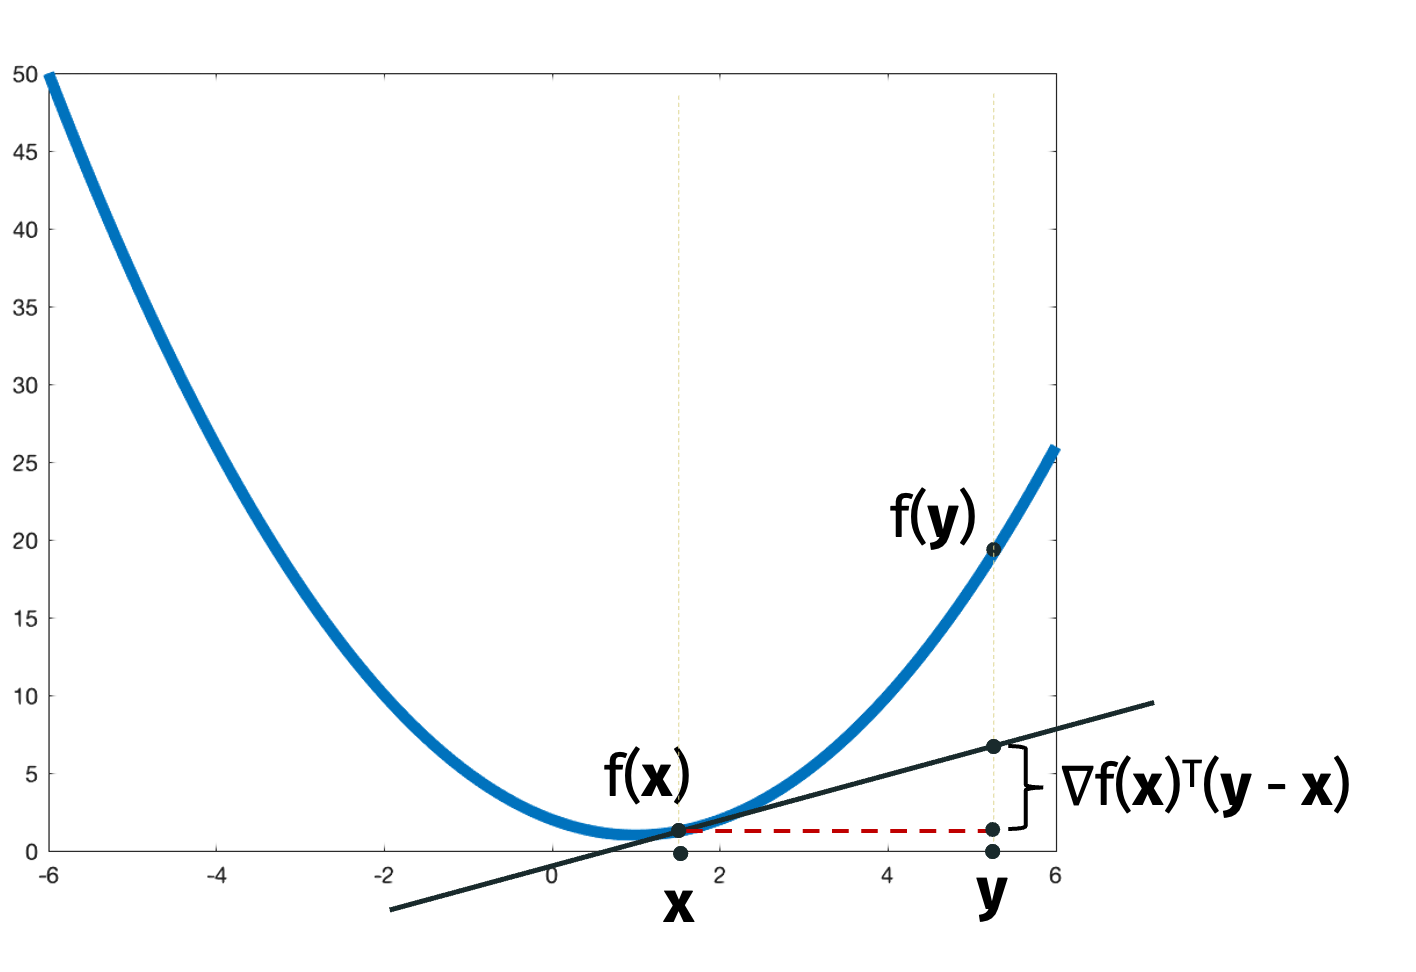
\includegraphics[width=.6\textwidth]{smoothness_image.png}

	\textbf{We will discuss and analyzing this setting after the midterm!}
\end{center}	
\end{frame}

% \begin{frame}[t]
% 	\frametitle{convergence guarantee}
% 	\begin{align*}
% 		\alert{\frac{\alpha}{2}}\|\bv{x} - \bv{y}\|_2^2 \leq\left[f(\bv{y}) - f(\bv{x})\right] - \nabla f(\bv{x})^T(\bv{y} - \bv{x}) \leq \alert{\frac{\beta}{2}}\|\bv{x} - \bv{y}\|_2^2.
% 	\end{align*}
	
% 	\begin{theorem}[GD for $\beta$-smooth, $\alpha$-strongly convex.]
% 		Let $f$ be a $\beta$-smooth and $\alpha$-strongly convex function. If we run GD for $T$ steps (with step size $\eta = \frac{1}{\beta}$) we have:
% 		\begin{align*}
% 			\|\bv{x}^{(T)} - \bv{x}^*\|_2^2 \leq e^{-T \frac{\alpha}{\beta}} \|\bv{x}^{(0)} - \bv{x}^*\|_2^2
% 		\end{align*} 
% 	\end{theorem}	
% 	\begin{center}
% 		\alert{$\kappa = \frac{\beta}{\alpha}$} is called the ``condition number'' of $f$. 
		
% 		\textbf{Is it better if $\kappa$ is large or small?}
% 	\end{center}
% \end{frame}

% \begin{frame}[t]
% 	\frametitle{smooth and strongly convex}
% 	\textbf{Converting to more familiar form:}
% 	Using that fact the $\nabla f(\bv{x}^*) = \bv{0}$ along with
% 	\begin{align*}
% 		{\frac{\alpha}{2}}\|\bv{x} - \bv{y}\|_2^2 \leq  \left[f(\bv{y}) - f(\bv{x})\right] - \nabla f(\bv{x})^T(\bv{y} - \bv{x}) \leq {\frac{\beta}{2}}\|\bv{x} - \bv{y}\|_2^2, 
% 	\end{align*}
% 	we have:
% 	\begin{align*}
% 		\|\bv{x}^{(1)} - \bv{x}^*\|_2^2 &\leq \frac{2}{\alpha} \left[f(\bv{x}^{(0)}) - f(\bv{x}^*)\right]\\
% 		\|\bv{x}^{(T)} - \bv{x}^*\|_2^2 &\geq \frac{2}{\beta} \left[f(\bv{x}^{(T)}) - f(\bv{x}^*)\right]
% 	\end{align*}	
% \end{frame}

% \begin{frame}[t]
% 	\frametitle{convergence guarantee}
% 	\begin{corollary}[GD for $\beta$-smooth, $\alpha$-strongly convex.]
% 		Let $f$ be a $\beta$-smooth and $\alpha$-strongly convex function. If we run GD for $T$ steps (with step size $\eta = \frac{1}{\beta}$) we have:
% 		\begin{align*}
% 			f(\bv{x}^{(T)}) - f(\bv{x}^*)  \leq \frac{\beta}{\alpha} e^{-T\frac{\alpha}{\beta}} \cdot  \left[f(\bv{x}^{(0)}) - f(\bv{x}^*)\right]
% 		\end{align*} 
% 	\end{corollary}	
	
% 	\textbf{Corollary}: 
% 	If \alert{$T = O\left(\frac{\beta}{\alpha}\log(\beta/\alpha \epsilon)\right) =  O(\kappa\log(\kappa/\epsilon))$ } we have:
% 	\begin{align*}
% 		f({\bv{x}}^{(T)}) - f(\bv{x}^*) \leq \epsilon \left[f(\bv{x}^{(0)}) - f(\bv{x}^*)\right]
% 	\end{align*}
	
% 	\textbf{Alternative Corollary}: 
% 	If \alert{$T = O\left(\frac{\beta}{\alpha}\log(R\beta/\epsilon)\right)$} we have:
% 	\begin{align*}
% 		f({\bv{x}}^{(T)}) - f(\bv{x}^*) \leq \epsilon
% 	\end{align*}
% 	Only depend on $\log(1/\epsilon)$ instead of on $1/\epsilon$ or $1/\epsilon^2$!
% \end{frame}

% \begin{frame}[t]
% 	\frametitle{all convergence guarantees}
% 	Convexity: 
% 	\begin{align*}
% 		0 \leq \left[f(\bv{y}) - f(\bv{x})\right] - \nabla f(\bv{x})^T(\bv{y} - \bv{x})
% 	\end{align*}
% 	$\alpha$-strong-convexity and $\beta$-smoothness:
% 	\begin{align*}
% 		\alert{\frac{\alpha}{2}}\|\bv{x} - \bv{y}\|_2^2 \leq\left[f(\bv{y}) - f(\bv{x})\right] - \nabla f(\bv{x})^T(\bv{y} - \bv{x}) \leq \alert{\frac{\beta}{2}}\|\bv{x} - \bv{y}\|_2^2.
% 	\end{align*}
% 	\textbf{Number of iterations for $\epsilon$ error:}
% 	\begin{center}
% 		\begin{tabular}{c|cc}
% 			& $G$-Lipschitz & $\beta$-smooth   \\ \hline
% 			$R$ bounded start & $O\left(\frac{G^2R^2}{\epsilon^2}\right)$ & $O\left(\frac{\beta R^2}{\epsilon}\right)$ \\
% 			$\alpha$-strong convex & $O\left(\frac{G^2}{\alpha\epsilon}\right)$ & $O\left(\frac{\beta}{\alpha}\log(1/\epsilon)\right)$
% 		\end{tabular}
% 	\end{center}
	
% \end{frame}

% \begin{frame}[t]
% 	\frametitle{the hessian}
% 	Let $f$ be a twice differentiable function from $\R^d \rightarrow \R$. Let the \textbf{\alert{Hessian}} $\bv{H} = \nabla^2 f(\bv{x})$ contain all of its second derivatives at a point $\bv{x}$. So $\bv{H}\in \R^{d\times d}$.  We have:
% 	\begin{align*}
% 		\bv{H}_{j,k} = \left[\nabla^2 f(\bv{x})\right]_{j,k} = \frac{\partial^2 f}{\partial x_j x_k}. 
% 	\end{align*}
	
% 	For vector $\bv{x}, \bv{v}$:
% 	\begin{align*}
% 		\nabla f(\bv{x} + t\bv{v}) \approx \nabla f(\bv{x}) + t\left[\nabla^2 f(\bv{x})\right]\bv{v}.
% 	\end{align*}
% \end{frame}

% \begin{frame}[t]
% 	\frametitle{the hessian}
% 	Let $f$ be a twice differentiable function from $\R^d \rightarrow \R$. Let the \textbf{\alert{Hessian}} $\bv{H} = \nabla^2 f(\bv{x})$ contain all of its second derivatives at a point $\bv{x}$. So $\bv{H}\in \R^{d\times d}$.  We have:
% 	\begin{align*}
% 		\bv{H}_{j,k} = \left[\nabla^2 f(\bv{x})\right]_{j,k} = \frac{\partial^2 f}{\partial x_j x_k}. 
% 	\end{align*}
	
% 	\textbf{Example:} $f(\bv{x}) = \sum_{i=1}^n \left(\bv{x}^T\bv{a}^{(i)} - {y}^{(i)}\right)^2 = \|\bv{A}\bv{x} - \bv{y}\|_2^2$
% 	\begin{align*}
% 		\frac{\partial f}{\partial x_j} &= \sum_{i=1}^n 2\left(\bv{x}^T\bv{a}^{(i)} - {y}^{(i)}\right)\cdot a^{(i)}_j \\
% 		\frac{\partial^2 f}{\partial x_k\partial x_j} &= \sum_{i=1}^n 2a^{(i)}_k  a^{(i)}_j \\
% 		\bv{H} &=  
% 	\end{align*}
% \end{frame}



% \begin{frame}[t]
% 	\frametitle{alternative derivation}
% 	$f(\bv{x}) = \|\bv{A}\bv{x} - \bv{b}\|_2^2$. Recall that $\nabla f(\bv{x}) = 2\bv{A}^T(\bv{A}\bv{x}-\bv{b}).$
	
% \end{frame}

% \begin{frame}[t]
% 	\frametitle{hessian matrices and positive semidefiniteness}
% 	\textbf{Claim:} If $f$ is twice differentiable, then it is convex if and only if the matrix $\bv{H} = \nabla^2 f(\bv{x})$ is \emph{positive semidefinite} for all $\bv{x}$. 
	
% 	\begin{definition}[Positive Semidefinite (PSD)]
% 		A square, symmetric matrix $\bv{H}\in \R^{d\times d}$ is \emph{positive semidefinite} (PSD) for any vector $\bv{y}\in \R^d$, $\bv{y}^T\bv{H}\bv{y} \geq 0$. 
% 	\end{definition}
	
% 	This is a natural notion of ``positivity'' for symmetric matrices. To denote that $\bv{H}$ is PSD we will typically use ``Loewner order'' notation (\texttt{\textbackslash succeq} in LaTex): $$\bv{H}\succeq 0.$$
	
% 	We write $\bv{B}\succeq \bv{A}$ or equivalently  $\bv{A}\preceq \bv{B}$ to denote that $(\bv{B} - \bv{A})$ is positive semidefinite. This gives a \emph{partial ordering} on matrices.
% \end{frame}

% \begin{frame}[t]
% 	\frametitle{hessian matrices and positive semidefiniteness}
% 	\textbf{Claim:} If $f$ is twice differentiable, then it is convex if and only if the matrix $\bv{H} = \nabla^2 f(\bv{x})$ is \emph{positive semidefinite} for all $\bv{x}$. 
	
% 	\begin{definition}[Positive Semidefinite (PSD)]
% 		A square, symmetric matrix $\bv{H}\in \R^{d\times d}$ is \emph{positive semidefinite} (PSD) for any vector $\bv{y}\in \R^d$, $\bv{y}^T\bv{H}\bv{y} \geq 0$. 
% 	\end{definition}
	
% 	For the least squares regression loss function: $f(\bv{x}) = \|\bv{A}\bv{x} - \bv{b}\|_2^2$, $\bv{H} = \nabla^2 f(\bv{x})= 2\bv{A}^T\bv{A}$ for all $\bv{x}$. Is $\bv{H}$ PSD?
% \end{frame}

% \begin{frame}[t]
% 	\frametitle{the linear algebra of conditioning}
% 	If $f$ is $\beta$-smooth and $\alpha$-strongly convex then at any point $\bv{x}$, $\bv{H} = \nabla^2 f(\bv{x})$ satisfies: 
% 	\begin{align*}
% 		\alpha\bv{I}\preceq \bv{H} \preceq \beta\bv{I},
% 	\end{align*}
% 	where $\bv{I}$ is a $d\times d$ identity matrix. 
	
% 	This is the natural matrix generalization of the statement for scalar valued functions:
% 	\begin{align*}
% 		\alpha \leq f''(x)\leq \beta.
% 	\end{align*}
	
% \end{frame}

% \begin{frame}[t]
% 	\frametitle{smooth and strongly convex hessian}
% 	\begin{align*}
% 		\alpha\bv{I}_{d\times d} \preceq \bv{H} \preceq \beta\bv{I}_{d\times d}.
% 	\end{align*}
% 	Equivalently for any $\bv{z}$,
% 	\begin{align*}
% 		\alpha\|\bv{z}\|_2^2 \leq \bv{z}^T\bv{H}\bv{z} \leq \beta\|\bv{z}\|_2^2.
% 	\end{align*} 
% \end{frame}

% \begin{frame}[t]
% 	\frametitle{simple example}
% 	Let $f(\bv{x}) = \|\bv{D}\bv{x} - \bv{b}\|_2^2$ where $\bv{D}$ is a diagaonl matrix. For now imagine we're in two dimensions: $\bv{x} = \begin{bmatrix}
% 		x_1\\
% 		x_2
% 	\end{bmatrix}$, $\bv{D} = \begin{bmatrix}
% 		d_1 & 0 \\
% 		0 & d_2
% 	\end{bmatrix}
% 	$.
% 	\begin{center}
% 		\textbf{What are $\alpha,\beta$ for this problem?}
% 	\end{center}
% 	\begin{align*}
% 		\alpha\|\bv{z}\|_2^2 \leq \bv{z}^T\bv{H}\bv{z} \leq \beta\|\bv{z}\|_2^2
% 	\end{align*}
% \end{frame}

% \begin{frame}[t]
% 	\frametitle{geometric view}
% 	\begin{center}
% 		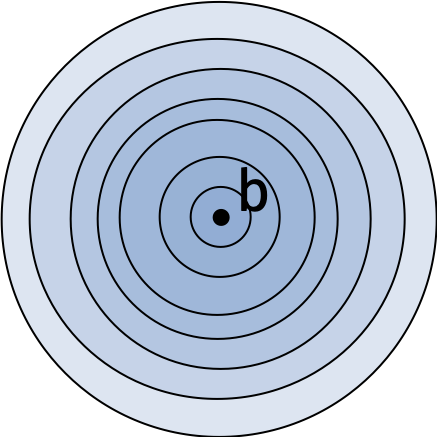
\includegraphics[width=.5\textwidth]{perfect_conditioning.png}
		
% 		Level sets of $\|\bv{D}\bv{x} - \bv{b}\|_2^2$ when $d_1^2 = 1, d_2^2 = 1$. 
% 	\end{center}
% \end{frame}

% \begin{frame}[t]
% 	\frametitle{geometric view}
% 	\begin{center}
% 		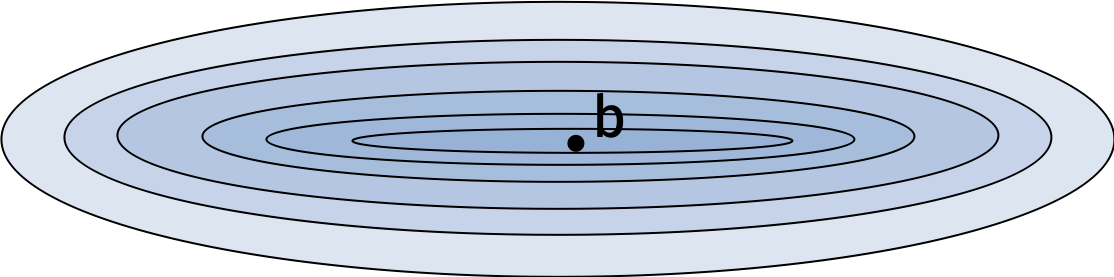
\includegraphics[width=\textwidth]{poor_conditioning.png}
		
% 		Level sets of $\|\bv{D}\bv{x} - \bv{b}\|_2^2$ when $d_1^2 = \frac{1}{3}, d_2^2 = 2$. 
% 	\end{center}
% \end{frame}

%\begin{frame}[t]
%	\frametitle{eigendecomposition view}
%	Any symmetric matrix $\bv{H}$ has an \emph{orthogonal}, real valued eigendecomposition. 
%	\begin{center}
%		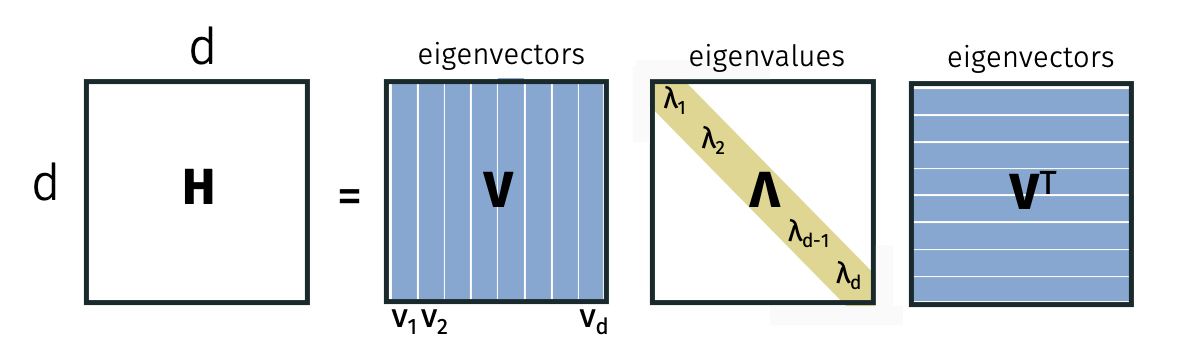
\includegraphics[width=.9\textwidth]{eigendecomp.png}
%	\end{center}
%	Here $\bv{V}$ is square and orthogonal, so $\bv{V}^T\bv{V} = \bv{V}\bv{V}^T = \bv{I}$. And for each $\bv{v}_i$, we have:
%	\begin{align*}
%		\bv{H}\bv{v}_i = \lambda_i \bv{v}_i. 
%	\end{align*}
%	By definition, that's what makes $\bv{v}_1, \ldots, \bv{v}_d$ eigenvectors.	
%\end{frame}
%
%\begin{frame}[t]
%	\frametitle{eigendecomposition view}
%	Recall $\bv{V}\bv{V}^T = \bv{V}^T\bv{V} = \bv{I}$.
%	\begin{center}
%		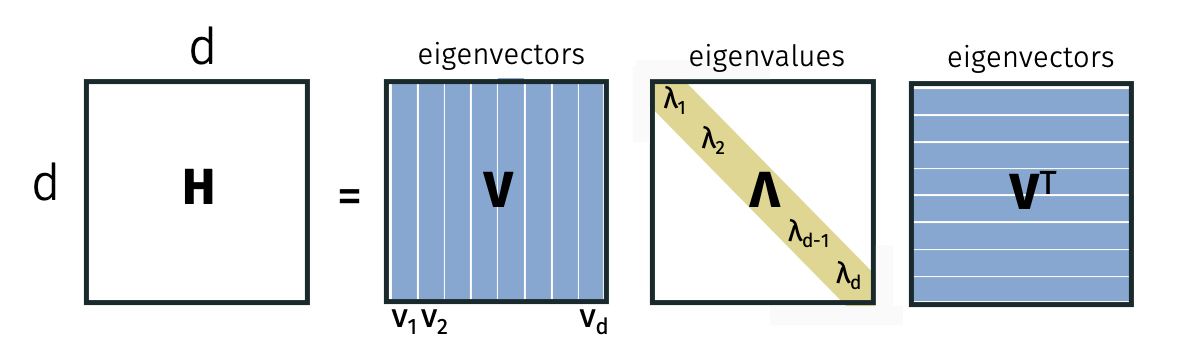
\includegraphics[width=.9\textwidth]{eigendecomp.png}
%	\end{center}
%	\textbf{Claim:}	$\bv{H} \text{ is PSD } \Leftrightarrow \lambda_1, ..., \lambda_d \geq 0$. 
%\end{frame}
%
%\begin{frame}[t]
%	\frametitle{eigendecomposition view}
%	Recall $\bv{V}\bv{V}^T = \bv{V}^T\bv{V} = \bv{I}$.
%	\begin{center}
%		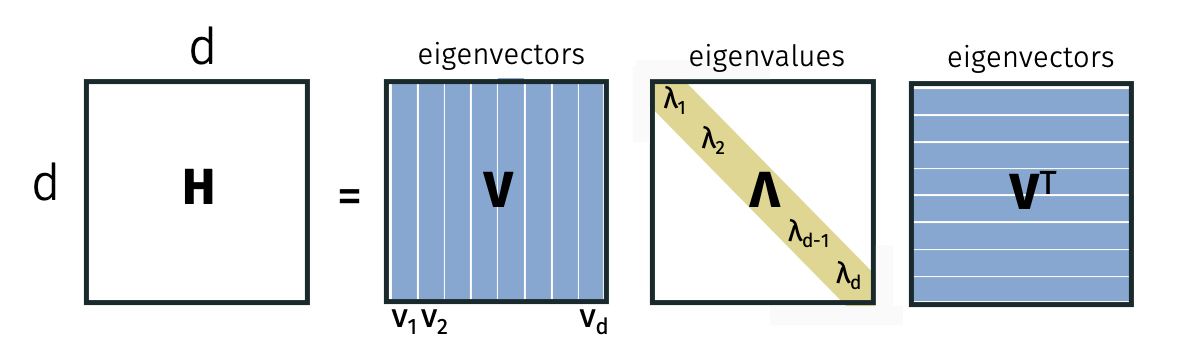
\includegraphics[width=.9\textwidth]{eigendecomp.png}
%	\end{center}
%	\textbf{Claim:}	$\alpha\bv{I} \preceq \bv{H} \preceq \beta \bv{I} \Leftrightarrow \alpha \leq \lambda_1, ..., \lambda_d \leq \beta$. 
%\end{frame}
%
%\begin{frame}[t]
%	\frametitle{eigendecomposition view}
%	Recall $\bv{V}\bv{V}^T = \bv{V}^T\bv{V} = \bv{I}$.
%	\begin{center}
%		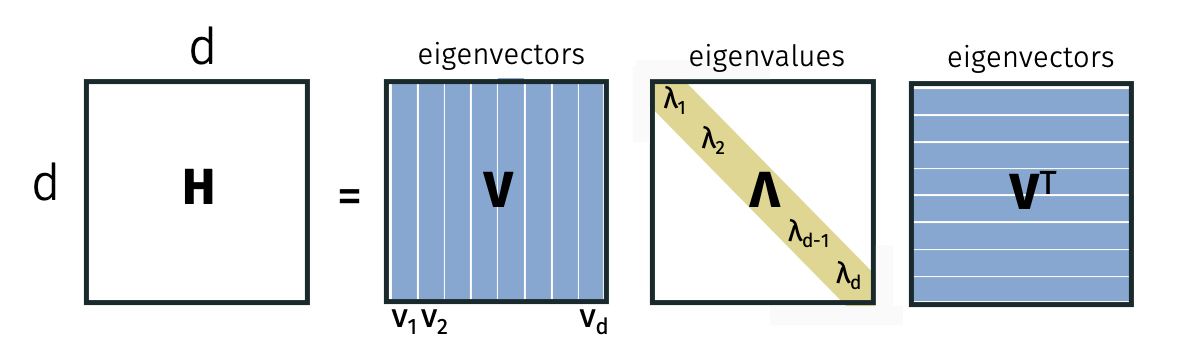
\includegraphics[width=.9\textwidth]{eigendecomp.png}
%	\end{center}
%	In other words, if we let $\lmax(\bv{H})$ and $\lmin(\bv{H})$ be the smallest and largest eigenvalues of $\bv{H}$, then for all $\bv{z}$ we have: 
%	\begin{align*}
%		\bv{z}^T\bv{H}\bv{z} &\leq \lmax(\bv{H})\cdot \|\bv{z}\|^2 \\
%		\bv{z}^T\bv{H}\bv{z} &\geq \lmin(\bv{H})\cdot \|\bv{z}\|^2 
%	\end{align*}
%	
%\end{frame}
%
%
%\begin{frame}[t]
%	\frametitle{eigendecomposition view}
%	If the maximum eigenvalue of $\bv{H} = \nabla^2f(\bv{x}) = \beta$ and the minimum eigenvalue of $\bv{H} = \nabla^2f(\bv{x}) = \alpha$ then $f(\bv{x})$ is $\beta$-smooth and $\alpha$-strongly convex.
%	
%	\begin{align*}
%		\lmax(\bv{H}) &= \beta\\
%		\lmin(\bv{H}) &= \alpha
%	\end{align*}
%\end{frame}
%
%\begin{frame}[t]
%	\frametitle{polynomial view point}
%	\begin{theorem}[GD for $\beta$-smooth, $\alpha$-strongly convex.]
%		Let $f$ be a $\beta$-smooth and $\alpha$-strongly convex function. If we run GD for $T$ steps (with step size $\eta = \frac{2}{\beta}$) we have:
%		\begin{align*}
%			\|\bv{x}^{(T)} - \bv{x}^*\|_2 \leq e^{-T/\kappa} \|\bv{x}^{(1)} - \bv{x}^*\|_2
%		\end{align*} 
%	\end{theorem}
%	
%	\begin{center}
%		\alert{\textbf{Goal: Prove for $f(\bv{x}) = \|\bv{A}\bv{x} - \bv{b}\|_2^2$.}}
%	\end{center}	
%Let $\lmax = \lmax(\bv{A}^T\bv{A})$. Gradient descent update is:
%\begin{align*}
%	\bv{x}^{(t+1)} = \bv{x}^{(t)} - \frac{1}{2\lmax}2\bv{A}^T(\bv{A}\bv{x}^{(t)} - \bv{b})
%\end{align*}
%
%\end{frame}
%
%\begin{frame}[t]
%	\frametitle{alternative view of gradient descent}
%	\textbf{Richardson Iteration view:}
%	\begin{align*}
%		(\bv{x}^{(t+1)} - \bv{x}^*) =  \left(\bv{I} - \frac{1}{\lmax}\bv{A}^T\bv{A}\right)(\bv{x}^{(t)} - \bv{x}^*) 
%	\end{align*}
%	
%	
%	\vspace{10em}
%	What is the maximum eigenvalue of the symmetric matrix $\left(\bv{I} - \frac{1}{\lmax}\bv{A}^T\bv{A}\right)$ in terms of the eigenvalues $\lmax = \lambda_1 \geq \ldots \geq \lambda_d = \lmin$ of $\bv{A}^T\bv{A}$?
%\end{frame}
%
%\begin{frame}[t]
%	\frametitle{unrolled gradient descent}
%	\begin{align*}
%		(\bv{x}^{(T+1)} - \bv{x}^*) =  \left(\bv{I} - \frac{1}{\lmax}\bv{A}^T\bv{A}\right)^T(\bv{x}^{(1)} - \bv{x}^*) 
%	\end{align*}
%	
%	\vspace{3em}
%	What is the maximum eigenvalue of the symmetric matrix $\left(\bv{I} - \frac{1}{\lmax}\bv{A}^T\bv{A}\right)^T$?
%	
%	\vspace{5em}
%	So we have $\|\bv{x}^{(T)} - \bv{x}^*\|_2 \leq $
%\end{frame}
%
%\begin{frame}
%	\frametitle{improving gradient descent}
%	We now have a pretty good understanding of gradient descent. 
%	
%	\textbf{Number of iterations for $\epsilon$ error:}
%	\begin{center}
%		\begin{tabular}{c|cc}
%			& $G$-Lipschitz & $\beta$-smooth   \\ \hline
%			$R$ bounded start & $O\left(\frac{G^2R^2}{\epsilon^2}\right)$ & $O\left(\frac{\beta R^2}{\epsilon}\right)$ \\
%			$\alpha$-strong convex & $O\left(\frac{G^2}{\alpha\epsilon}\right)$ & $O\left(\frac{\beta}{\alpha}\log(1/\epsilon)\right)$
%		\end{tabular}
%	\end{center}
%	
%%	\vspace{1em}
%%	\alert{How do we use this understanding to design \emph{faster algorithms?}}
%\end{frame}
%
%\begin{frame}[standout]
%	\begin{center}
%		\large acceleration
%	\end{center}
%\end{frame}
%
%
%\begin{frame}
%	\frametitle{accelerated gradient descent}
%	\textbf{Nesterov's accelerated gradient descent}:
%	\begin{itemize}
%		\item $\bv{x}^{(1)} = \bv{y}^{(1)} = \bv{z}^{(1)}$  
%		\item For $t = 1,\ldots, T$
%		\begin{itemize}
%			\item $\bv{y}^{(t+1)} = \bv{x}^{(t)} - \frac{1}{\beta}\nabla f(\bv{x}^{(t)})$
%			\item $\bv{x}^{(t+1)} = \left(1 + \frac{\sqrt{\kappa} - 1}{\sqrt{\kappa} + 1}\right) \bv{y}^{(t+1)} + \frac{\sqrt{\kappa} - 1}{\sqrt{\kappa} + 1}\left(\bv{y}^{(t+1)} - \bv{y}^{(t)}\right)$
%		\end{itemize}
%	\end{itemize}
%	\begin{theorem}[AGD for $\beta$-smooth, $\alpha$-strongly convex.]
%		Let $f$ be a $\beta$-smooth and $\alpha$-strongly convex function. If we run AGD for $T$ steps we have:
%		\begin{align*}
%			f(\bv{x}^{(t)}) - f(\bv{x}^*) \leq \kappa e^{-(t-1)\sqrt{\kappa}} \left[f(\bv{x}^{(1)}) - f(\bv{x}^*) \right]
%		\end{align*} 
%	\end{theorem}	
%	\textbf{Corollary:} If \alert{$T = O\left(\sqrt{\kappa}\log(\kappa/\epsilon)\right)$ achieve error $\epsilon$.} 
%	
%\end{frame}
%
%\begin{frame}[t]
%	\frametitle{linear regression runtime}
%	\textbf{Total runtime for solving linear regression via GD}:
%	\begin{center}
%		(time per iteration) x (number of iterations)
%		
%		\vspace{5em}
%		
%		\large
%		$\alert{O(nd\cdot\kappa\log(1/\epsilon))}$
%		
%		for $\bv{A}\in \R^{n\times d}$, $\bv{x} \in \R^d$, $\bv{b}\in \R^n$.
%	\end{center}	
%\end{frame}
%
%\begin{frame}[t]
%	\frametitle{acceleration}
%	\begin{theorem}[Accelerated Iterative Regression]
%		Let $\bv{x}^* = \min_{\bv{x}}\|\bv{A}\bv{x} - \bv{b}\|_2^2$. There is an algorithm which finds $\tilde{\bv{x}} $ with $\|\tilde{\bv{x}} - \bv{x}^*\|_2 \leq \epsilon\|\bv{x}^*\|_2$ in time:
%			\begin{align*}
%				O(nd\cdot\sqrt{\kappa\log(1/\epsilon)})
%			\end{align*} 
%	\end{theorem}
%\end{frame}
%
%\begin{frame}[t]
%	\frametitle{the polynomial view}
%	\textbf{Claim:} For any $\eta$, polynomial $p(z) = c_1 z + c_2 z^2 + \ldots + c_q z^q$ with $p(1) = \sum_{j=1}^q c_q = 1$, there is an algorithm running in $O(ndq)$ time which outputs $\tilde{\bv{x}}$ satisfying:
%	\begin{align*}
%	\tilde{\bv{x}} - \bv{x}^* =  p(\bv{I} - \frac{1}{\eta}\bv{A}^T\bv{A}) \bv{x}^*
%	\end{align*}
%	
%	\begin{center}
%		\alert{For standard gradient descent, $p(z) = z^q$.}
%	\end{center}
%\end{frame}
%
%\begin{frame}[t]
%	\frametitle{the polynomial view}
%	\textbf{Claim:} For any $\eta$, polynomial $p(z) = c_1 z + c_2 z^2 + \ldots + c_q z^q$ with $p(1) = \sum_{j=1}^q c_q = 1$, there is an algorithm running in $O(ndq)$ time which outputs $\tilde{\bv{x}}$ satisfying:
%	\begin{align*}
%	\tilde{\bv{x}} - \bv{x}^* =  c_1\cdot (\bv{I} - \eta\bv{A}^T\bv{A})\bv{x}^* + c_2 \cdot (\bv{I} - \eta\bv{A}^T\bv{A})^2  \bv{x}^* + \ldots + c_q \cdot (\bv{I} - \eta\bv{A}^T\bv{A})^q  \bv{x}^* 
%	\end{align*}
%	
%	\textbf{Claim:} $c_j  \cdot \bv{I} - \eta\bv{A}^T\bv{A})^j\bv{x}^* = c_j\cdot\bv{x}^* + p_j'(\bv{I} - \eta\bv{A}^T\bv{A})\bv{A}^T\bv{A}\bv{x}^*$ where $p_j$ is a polynomial with degree $j - 1$.
%\end{frame}
%
%\begin{frame}[t]
%	\frametitle{the polynomial view}
%	\textbf{Claim:} For any $\eta$, polynomial $p(z) = c_1 z + c_2 z^2 + \ldots + c_q z^q$ with $p(1) = \sum_{j=1}^q c_q = 1$, there is an algorithm running in $O(ndq)$ time which outputs $\tilde{\bv{x}}$ satisfying:
%	\begin{align*}
%	\bv{x}^* - \tilde{\bv{x}} &=  (c_1 + c_2 + \ldots + c_q)\cdot\bv{x}^* +  p'(\bv{I} - \eta\bv{A}^T\bv{A})\bv{A}^T\bv{A}\bv{x}^*
%	\end{align*}
%	\begin{align*}
%		\tilde{\bv{x}}  &= p'(\bv{I} - \eta\bv{A}^T\bv{A})\bv{A}^T\bv{b} \text{ where $p'$ is a polynmial with degree $q-1$}.
%	\end{align*}
%\end{frame}
%
%\begin{frame}[t]
%	\frametitle{the polynomial view}
%	\begin{align*}
%	\tilde{\bv{x}} - \bv{x}^* =  p(\bv{I} - \eta\bv{A}^T\bv{A})\bv{x}^*\\
%	p(\bv{I} - \eta\bv{A}^T\bv{A}) = \bv{U}p(\bv{I} - \eta\bs{\Lambda})\bv{U}^T
%	\end{align*}
%	
%	\begin{align*}
%	\|\tilde{\bv{x}} - \bv{x}^*\|  &= \|\bv{U}p(\bv{I} - \eta\bs{\Lambda})\bv{U}^T\bv{x}^*\|_2 \\
%	& = \|p(\bv{I} - \eta\bs{\Lambda})\bv{U}^T\bv{x}^*\|_2
%	\end{align*}
%	
%	As long as $\max\left[ p(\bv{I} - \eta\bs{\Lambda})\right] \leq \epsilon$, 
%	\begin{align*}
%	\|\tilde{\bv{x}} - \bv{x}^*\|_2  \leq \epsilon \|\bv{x}^*\|_2 
%	\end{align*}
%\end{frame}
%
%\begin{frame}[t]
%	\frametitle{constructing a jump polynomial}
%	\textbf{Goal:} Find polynomial $p$ such that $p(1) = 1$ and $p(z) \leq \epsilon$ for $z\in [0,1 - \frac{1}{\kappa}]$.
%	\begin{center}
%		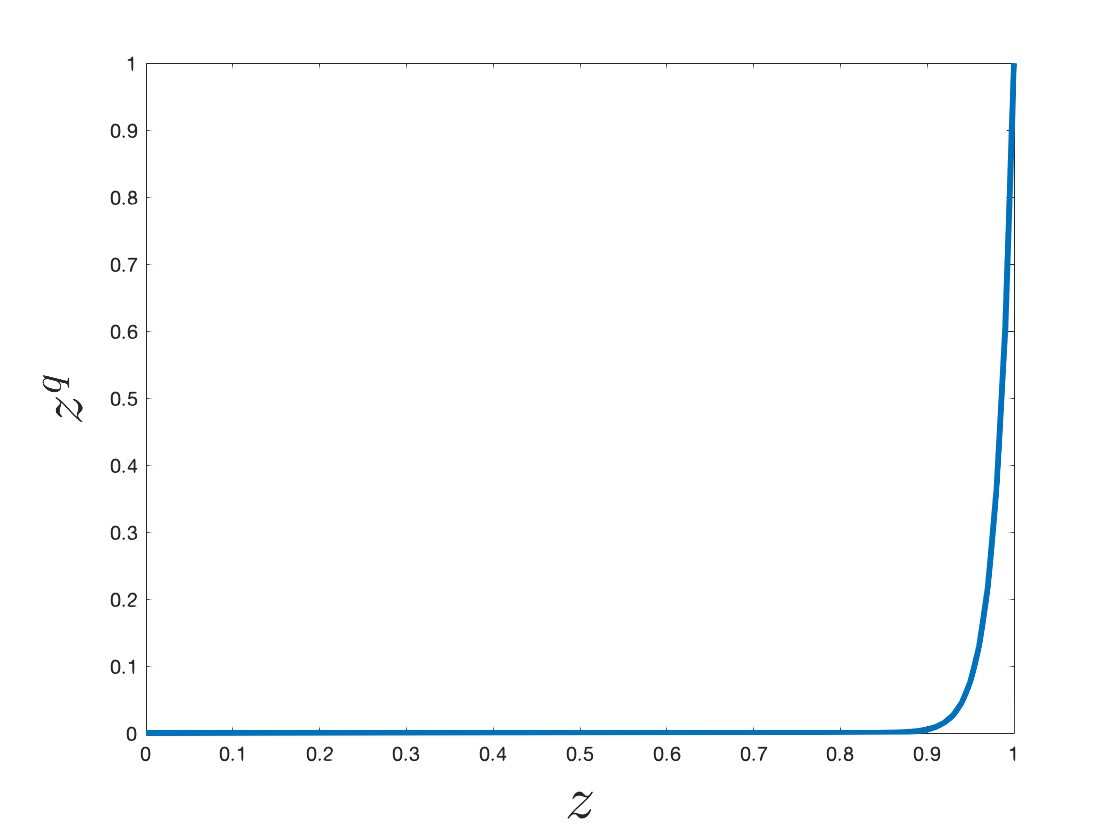
\includegraphics[width=.6\textwidth]{basic_jump.png}
%		
%		Gradient descent uses $p(z) = z^{O(\kappa\log(1/\epsilon))}$.
%	\end{center}
%\end{frame}
%
%\begin{frame}[t]
%	\frametitle{a better jump polynomial}
%		\textbf{Goal:} Find polynomial $p$ such that $p(1) = 1$ and $p(z) \leq \epsilon$ for $z\in [0,1 - \frac{1}{\kappa}]$.
%	\begin{center}
%		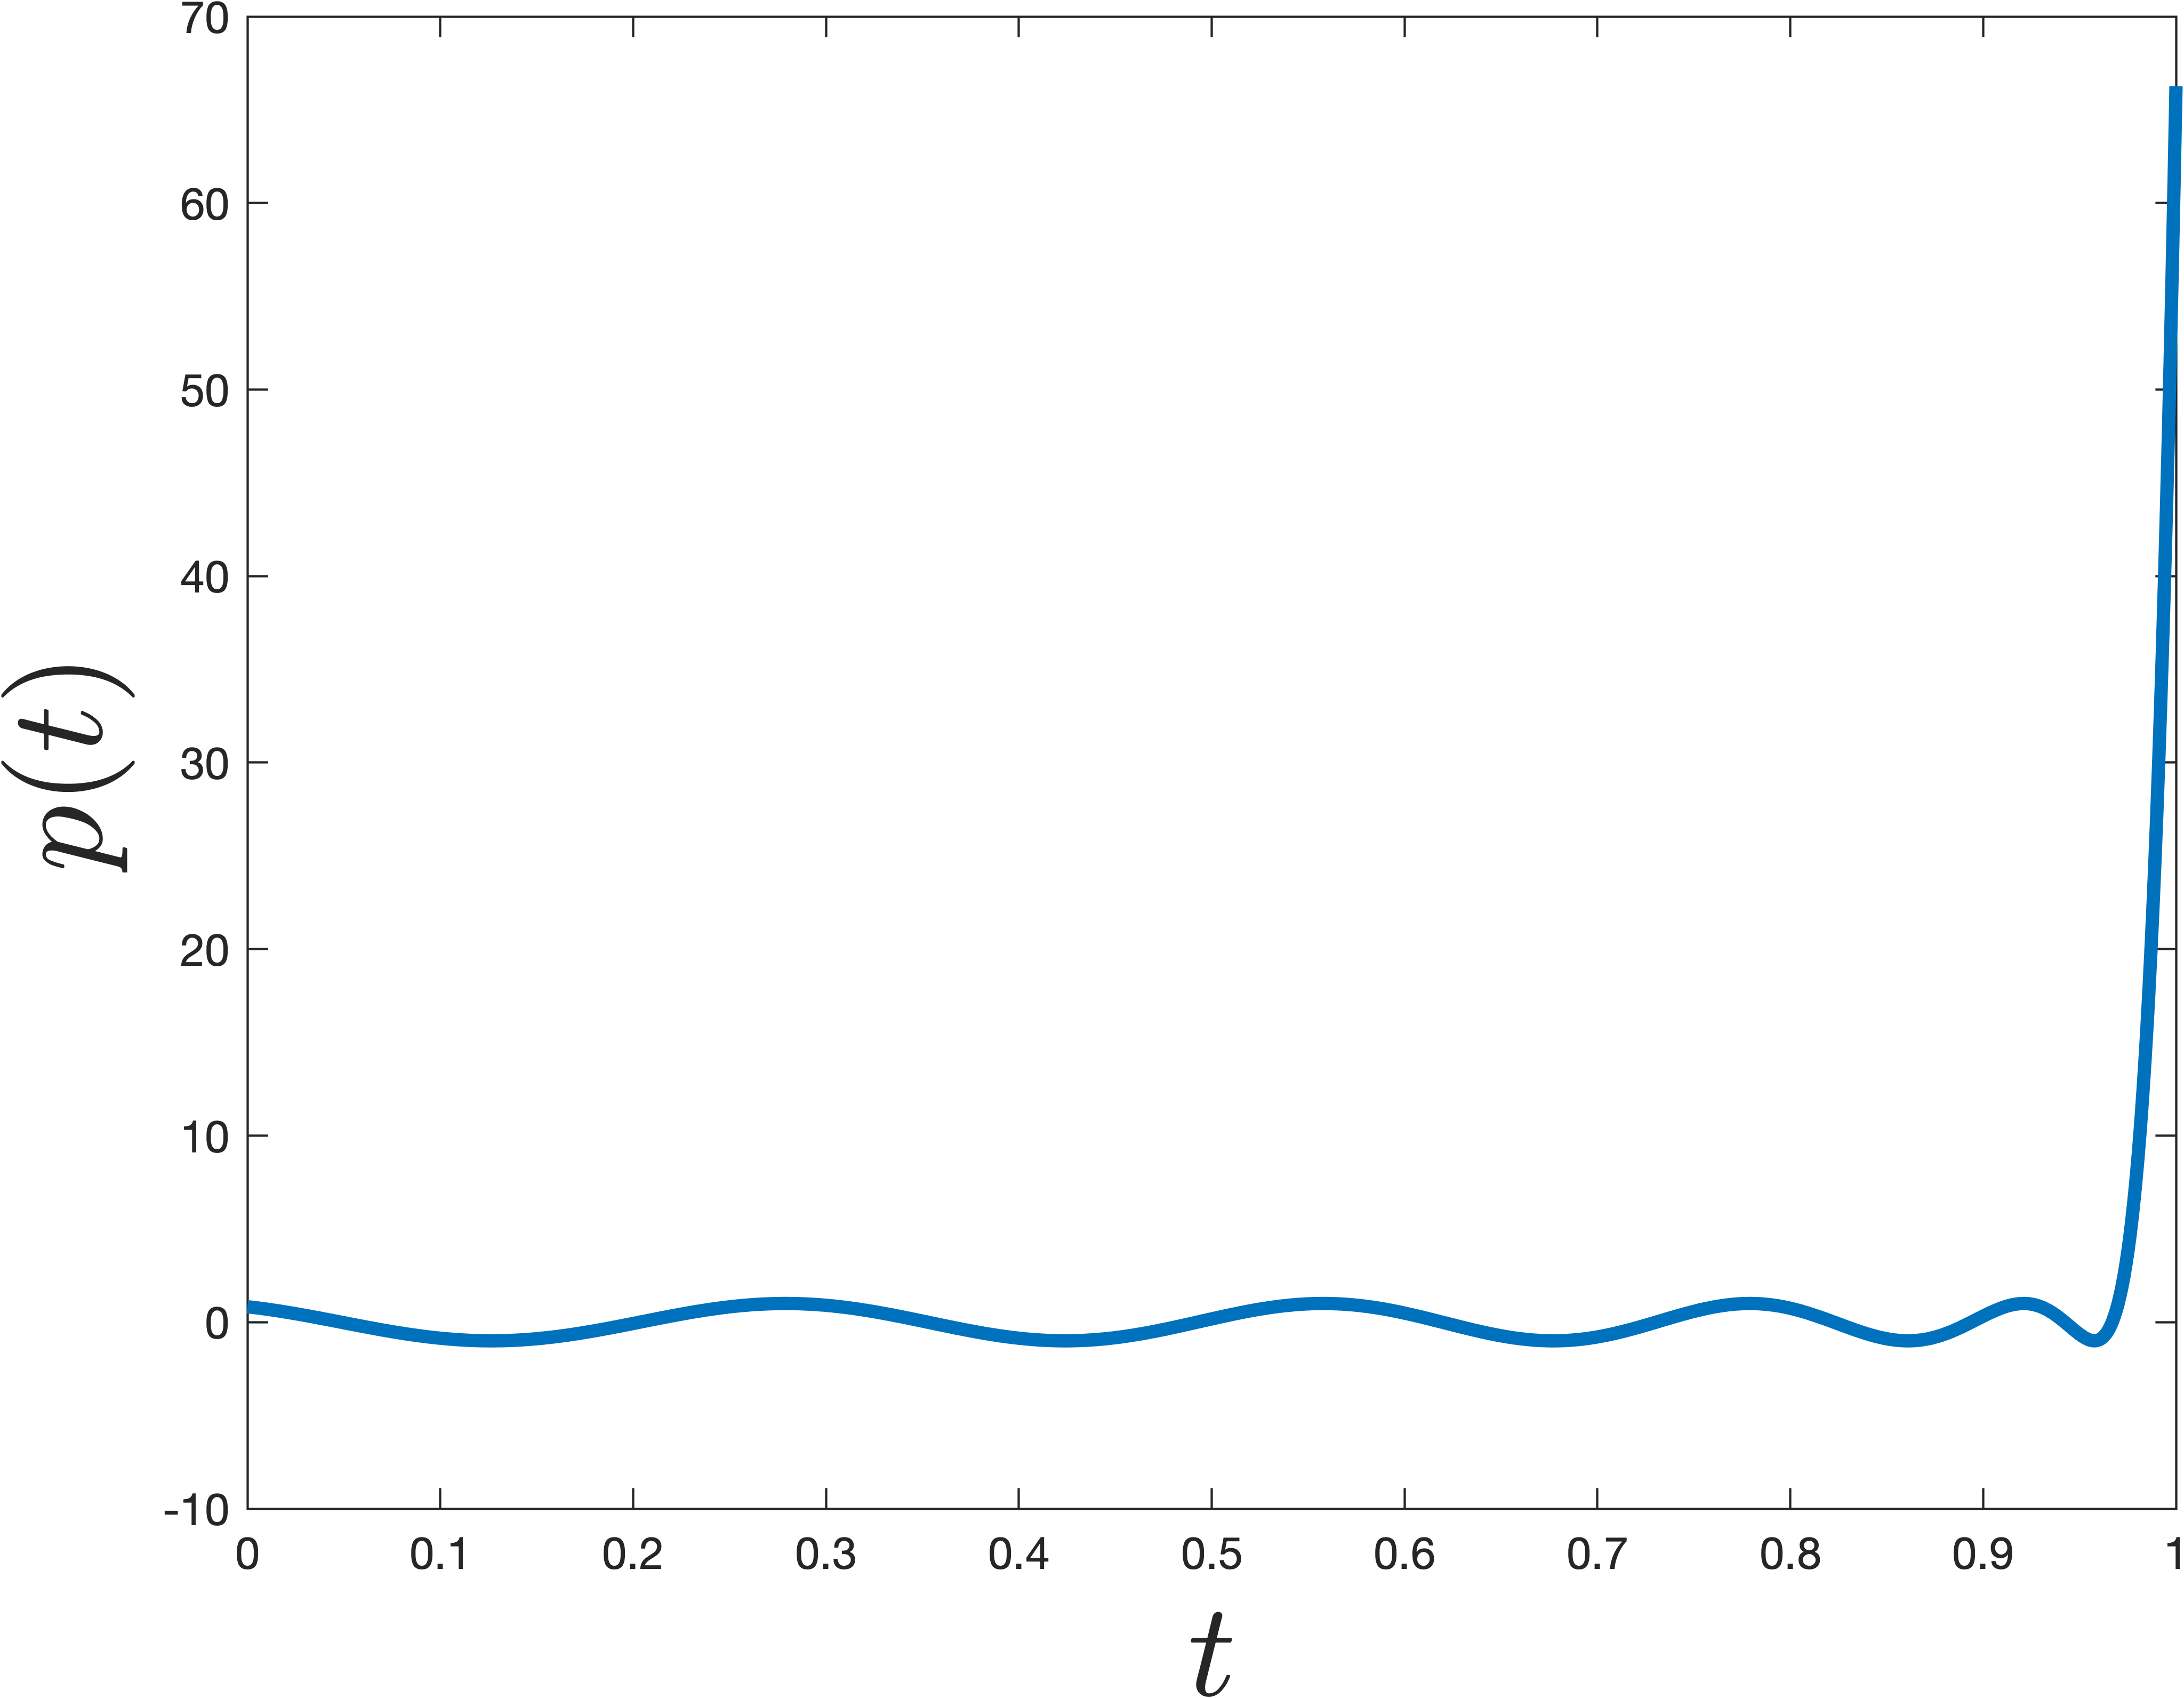
\includegraphics[width=.6\textwidth]{cheby_jump.png}
%		
%		\alert{Can be done with degree $O(\sqrt{\kappa\log(1/\epsilon)})$ polynomial instead!}
%	\end{center}
%\end{frame}
%
%\begin{frame}
%	\frametitle{chebyshev polynomials}
%	\begin{center}
%		\textbf{What are these polynomials?}
%	\end{center}
%	
%		\centering
%		Chebyshev polynomials of the first kind.
%		\begin{columns}
%			\begin{column}{0.5\textwidth}
%				\begin{align*}
%				T_0(x) &= 1\\
%				T_1(x) &= x \\
%				T_2(x) &= 2x^2 - 1\\
%				&\,\,\,\vdots\\
%				T_k(x) &= 2xT_{k-1}(x) - T_{k-2}(x)\\
%				\end{align*}
%			\end{column}
%			\begin{column}{0.5\textwidth}
%				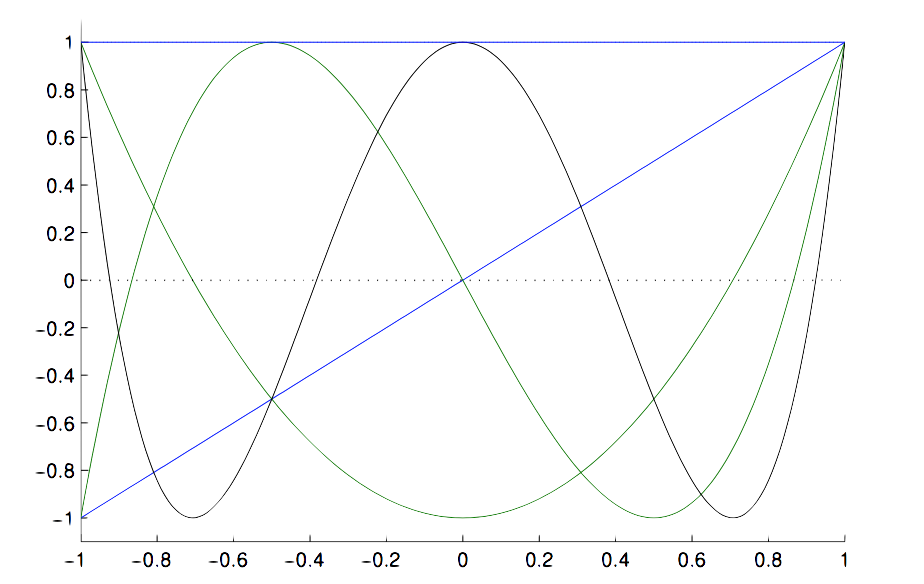
\includegraphics[width=\textwidth]{chebyPolys.png}
%			\end{column}
%		\end{columns}
%		\begin{center}
%			\textbf{``There's only one bullet in the gun. It's called the Chebyshev polynomial.''} -- Prof. Rocco Servedio
%		\end{center}
%\end{frame}
%
%\begin{frame}
%	\frametitle{accelerated gradient descent}
%	\textbf{Nesterov's accelerated gradient descent}:
%	\begin{itemize}
%		\item $\bv{x}^{(1)} = \bv{y}^{(1)} = \bv{z}^{(1)}$  
%		\item For $t = 1,\ldots, T$
%		\begin{itemize}
%			\item $\bv{y}^{(t+1)} = \bv{x}^{(t)} - \frac{1}{\beta}\nabla f(\bv{x}^{(t)})$
%			\item $\bv{x}^{(t+1)} = \left(1 + \frac{\sqrt{\kappa} - 1}{\sqrt{\kappa} + 1}\right) \bv{y}^{(t+1)} - \frac{\sqrt{\kappa} - 1}{\sqrt{\kappa} + 1}\bv{y}^{(t)}$
%		\end{itemize}
%	\end{itemize}
%	\begin{theorem}[AGD for $\beta$-smooth, $\alpha$-strongly convex.]
%	Let $f$ be a $\beta$-smooth and $\alpha$-strongly convex function. If we run AGD for $T$ steps we have:
%	\begin{align*}
%	f(\bv{x}^{(t)}) - f(\bv{x}^*) \leq \kappa e^{-(t-1)\sqrt{\kappa}} \left[f(\bv{x}^{(1)}) - f(\bv{x}^*) \right]
%	\end{align*} 
%\end{theorem}	
%\textbf{Corollary:} If \alert{$T = O\left(\sqrt{\kappa}\log(\kappa/\epsilon)\right)$ achieve error $\epsilon$.} 
%	
%\end{frame}

%\begin{frame}[t]
%	\frametitle{intuition behind acceleration}
%	\begin{center}
%		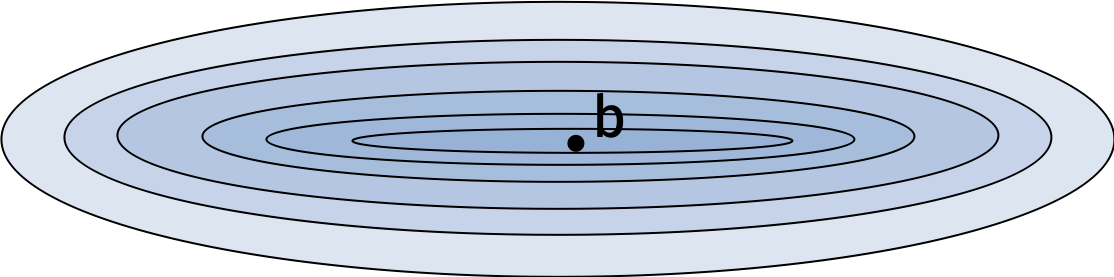
\includegraphics[width=\textwidth]{poor_conditioning.png}
%		
%		Level sets of $\|\bv{A}\bv{x} - \bv{b}\|_2^2$.
%	\end{center}
%	
%	\textbf{Other terms for similar ideas:}
%	\begin{itemize}
%		\item Momentum
%		\item Heavy-ball methods
%	\end{itemize}
%	
%	\begin{center}
%		\alert{What if we look back beyond \emph{two iterates}?}
%	\end{center}
%\end{frame}


\end{document} 








